
%% bare_conf.tex
%% V1.3
%% 2007/01/11
%% by Michael Shell
%% See:
%% http://www.michaelshell.org/
%% for current contact information.
%%
%% This is a skeleton file demonstrating the use of IEEEtran.cls
%% (requires IEEEtran.cls version 1.7 or later) with an IEEE conference paper.
%%
%% Support sites:
%% http://www.michaelshell.org/tex/ieeetran/
%% http://www.ctan.org/tex-archive/macros/latex/contrib/IEEEtran/
%% and
%% http://www.ieee.org/

%%*************************************************************************
%% Legal Notice:
%% This code is offered as-is without any warranty either expressed or
%% implied; without even the implied warranty of MERCHANTABILITY or
%% FITNESS FOR A PARTICULAR PURPOSE! 
%% User assumes all risk.
%% In no event shall IEEE or any contributor to this code be liable for
%% any damages or losses, including, but not limited to, incidental,
%% consequential, or any other damages, resulting from the use or misuse
%% of any information contained here.
%%
%% All comments are the opinions of their respective authors and are not
%% necessarily endorsed by the IEEE.
%%
%% This work is distributed under the LaTeX Project Public License (LPPL)
%% ( http://www.latex-project.org/ ) version 1.3, and may be freely used,
%% distributed and modified. A copy of the LPPL, version 1.3, is included
%% in the base LaTeX documentation of all distributions of LaTeX released
%% 2003/12/01 or later.
%% Retain all contribution notices and credits.
%% ** Modified files should be clearly indicated as such, including  **
%% ** renaming them and changing author support contact information. **
%%
%% File list of work: IEEEtran.cls, IEEEtran_HOWTO.pdf, bare_adv.tex,
%%                    bare_conf.tex, bare_jrnl.tex, bare_jrnl_compsoc.tex
%%*************************************************************************

% *** Authors should verify (and, if needed, correct) their LaTeX system  ***
% *** with the testflow diagnostic prior to trusting their LaTeX platform ***
% *** with production work. IEEE's font choices can trigger bugs that do  ***
% *** not appear when using other class files.                            ***
% The testflow support page is at:
% http://www.michaelshell.org/tex/testflow/



% Note that the a4paper option is mainly intended so that authors in
% countries using A4 can easily print to A4 and see how their papers will
% look in print - the typesetting of the document will not typically be
% affected with changes in paper size (but the bottom and side margins will).
% Use the testflow package mentioned above to verify correct handling of
% both paper sizes by the user's LaTeX system.
%
% Also note that the "draftcls" or "draftclsnofoot", not "draft", option
% should be used if it is desired that the figures are to be displayed in
% draft mode.
%
\documentclass[10pt, conference, compsocconf]{IEEEtran}
% Add the compsocconf option for Computer Society conferences.
%
% If IEEEtran.cls has not been installed into the LaTeX system files,
% manually specify the path to it like:
% \documentclass[conference]{../sty/IEEEtran}


\usepackage[tight,footnotesize]{subfigure}
\usepackage{calc}
\usepackage{amstext}
\usepackage[cmex10]{amsmath}
%\usepackage{amsthm}
%\usepackage{multicol}
\usepackage{pslatex}
\usepackage{color}
\usepackage{graphicx}
\usepackage[small]{caption}
\usepackage{booktabs}
%\usepackage{algorithm}
%\usepackage[noend]{algpseudocode}
\usepackage[linesnumbered]{algorithm2e}
\usepackage{epstopdf}
\usepackage{float}
\usepackage{flushend}

\newtheorem{theorem}{Theorem}
\newtheorem{corollary}{Corollary}[theorem]




% Some very useful LaTeX packages include:
% (uncomment the ones you want to load)


% *** MISC UTILITY PACKAGES ***
%
%\usepackage{ifpdf}
% Heiko Oberdiek's ifpdf.sty is very useful if you need conditional
% compilation based on whether the output is pdf or dvi.
% usage:
% \ifpdf
%   % pdf code
% \else
%   % dvi code
% \fi
% The latest version of ifpdf.sty can be obtained from:
% http://www.ctan.org/tex-archive/macros/latex/contrib/oberdiek/
% Also, note that IEEEtran.cls V1.7 and later provides a builtin
% \ifCLASSINFOpdf conditional that works the same way.
% When switching from latex to pdflatex and vice-versa, the compiler may
% have to be run twice to clear warning/error messages.






% *** CITATION PACKAGES ***
%
%\usepackage{cite}
% cite.sty was written by Donald Arseneau
% V1.6 and later of IEEEtran pre-defines the format of the cite.sty package
% \cite{} output to follow that of IEEE. Loading the cite package will
% result in citation numbers being automatically sorted and properly
% "compressed/ranged". e.g., [1], [9], [2], [7], [5], [6] without using
% cite.sty will become [1], [2], [5]--[7], [9] using cite.sty. cite.sty's
% \cite will automatically add leading space, if needed. Use cite.sty's
% noadjust option (cite.sty V3.8 and later) if you want to turn this off.
% cite.sty is already installed on most LaTeX systems. Be sure and use
% version 4.0 (2003-05-27) and later if using hyperref.sty. cite.sty does
% not currently provide for hyperlinked citations.
% The latest version can be obtained at:
% http://www.ctan.org/tex-archive/macros/latex/contrib/cite/
% The documentation is contained in the cite.sty file itself.






% *** GRAPHICS RELATED PACKAGES ***
%
\ifCLASSINFOpdf
  % \usepackage[pdftex]{graphicx}
  % declare the path(s) where your graphic files are
  % \graphicspath{{../pdf/}{../jpeg/}}
  % and their extensions so you won't have to specify these with
  % every instance of \includegraphics
  % \DeclareGraphicsExtensions{.pdf,.jpeg,.png}
\else
  % or other class option (dvipsone, dvipdf, if not using dvips). graphicx
  % will default to the driver specified in the system graphics.cfg if no
  % driver is specified.
  % \usepackage[dvips]{graphicx}
  % declare the path(s) where your graphic files are
  % \graphicspath{{../eps/}}
  % and their extensions so you won't have to specify these with
  % every instance of \includegraphics
  % \DeclareGraphicsExtensions{.eps}
\fi
% graphicx was written by David Carlisle and Sebastian Rahtz. It is
% required if you want graphics, photos, etc. graphicx.sty is already
% installed on most LaTeX systems. The latest version and documentation can
% be obtained at: 
% http://www.ctan.org/tex-archive/macros/latex/required/graphics/
% Another good source of documentation is "Using Imported Graphics in
% LaTeX2e" by Keith Reckdahl which can be found as epslatex.ps or
% epslatex.pdf at: http://www.ctan.org/tex-archive/info/
%
% latex, and pdflatex in dvi mode, support graphics in encapsulated
% postscript (.eps) format. pdflatex in pdf mode supports graphics
% in .pdf, .jpeg, .png and .mps (metapost) formats. Users should ensure
% that all non-photo figures use a vector format (.eps, .pdf, .mps) and
% not a bitmapped formats (.jpeg, .png). IEEE frowns on bitmapped formats
% which can result in "jaggedy"/blurry rendering of lines and letters as
% well as large increases in file sizes.
%
% You can find documentation about the pdfTeX application at:
% http://www.tug.org/applications/pdftex





% *** MATH PACKAGES ***
%
%\usepackage[cmex10]{amsmath}
% A popular package from the American Mathematical Society that provides
% many useful and powerful commands for dealing with mathematics. If using
% it, be sure to load this package with the cmex10 option to ensure that
% only type 1 fonts will utilized at all point sizes. Without this option,
% it is possible that some math symbols, particularly those within
% footnotes, will be rendered in bitmap form which will result in a
% document that can not be IEEE Xplore compliant!
%
% Also, note that the amsmath package sets \interdisplaylinepenalty to 10000
% thus preventing page breaks from occurring within multiline equations. Use:
%\interdisplaylinepenalty=2500
% after loading amsmath to restore such page breaks as IEEEtran.cls normally
% does. amsmath.sty is already installed on most LaTeX systems. The latest
% version and documentation can be obtained at:
% http://www.ctan.org/tex-archive/macros/latex/required/amslatex/math/





% *** SPECIALIZED LIST PACKAGES ***
%
%\usepackage{algorithmic}
% algorithmic.sty was written by Peter Williams and Rogerio Brito.
% This package provides an algorithmic environment fo describing algorithms.
% You can use the algorithmic environment in-text or within a figure
% environment to provide for a floating algorithm. Do NOT use the algorithm
% floating environment provided by algorithm.sty (by the same authors) or
% algorithm2e.sty (by Christophe Fiorio) as IEEE does not use dedicated
% algorithm float types and packages that provide these will not provide
% correct IEEE style captions. The latest version and documentation of
% algorithmic.sty can be obtained at:
% http://www.ctan.org/tex-archive/macros/latex/contrib/algorithms/
% There is also a support site at:
% http://algorithms.berlios.de/index.html
% Also of interest may be the (relatively newer and more customizable)
% algorithmicx.sty package by Szasz Janos:
% http://www.ctan.org/tex-archive/macros/latex/contrib/algorithmicx/




% *** ALIGNMENT PACKAGES ***
%
%\usepackage{array}
% Frank Mittelbach's and David Carlisle's array.sty patches and improves
% the standard LaTeX2e array and tabular environments to provide better
% appearance and additional user controls. As the default LaTeX2e table
% generation code is lacking to the point of almost being broken with
% respect to the quality of the end results, all users are strongly
% advised to use an enhanced (at the very least that provided by array.sty)
% set of table tools. array.sty is already installed on most systems. The
% latest version and documentation can be obtained at:
% http://www.ctan.org/tex-archive/macros/latex/required/tools/


%\usepackage{mdwmath}
%\usepackage{mdwtab}
% Also highly recommended is Mark Wooding's extremely powerful MDW tools,
% especially mdwmath.sty and mdwtab.sty which are used to format equations
% and tables, respectively. The MDWtools set is already installed on most
% LaTeX systems. The lastest version and documentation is available at:
% http://www.ctan.org/tex-archive/macros/latex/contrib/mdwtools/


% IEEEtran contains the IEEEeqnarray family of commands that can be used to
% generate multiline equations as well as matrices, tables, etc., of high
% quality.


%\usepackage{eqparbox}
% Also of notable interest is Scott Pakin's eqparbox package for creating
% (automatically sized) equal width boxes - aka "natural width parboxes".
% Available at:
% http://www.ctan.org/tex-archive/macros/latex/contrib/eqparbox/





% *** SUBFIGURE PACKAGES ***
%\usepackage[tight,footnotesize]{subfigure}
% subfigure.sty was written by Steven Douglas Cochran. This package makes it
% easy to put subfigures in your figures. e.g., "Figure 1a and 1b". For IEEE
% work, it is a good idea to load it with the tight package option to reduce
% the amount of white space around the subfigures. subfigure.sty is already
% installed on most LaTeX systems. The latest version and documentation can
% be obtained at:
% http://www.ctan.org/tex-archive/obsolete/macros/latex/contrib/subfigure/
% subfigure.sty has been superceeded by subfig.sty.



%\usepackage[caption=false]{caption}
%\usepackage[font=footnotesize]{subfig}
% subfig.sty, also written by Steven Douglas Cochran, is the modern
% replacement for subfigure.sty. However, subfig.sty requires and
% automatically loads Axel Sommerfeldt's caption.sty which will override
% IEEEtran.cls handling of captions and this will result in nonIEEE style
% figure/table captions. To prevent this problem, be sure and preload
% caption.sty with its "caption=false" package option. This is will preserve
% IEEEtran.cls handing of captions. Version 1.3 (2005/06/28) and later 
% (recommended due to many improvements over 1.2) of subfig.sty supports
% the caption=false option directly:
%\usepackage[caption=false,font=footnotesize]{subfig}
%
% The latest version and documentation can be obtained at:
% http://www.ctan.org/tex-archive/macros/latex/contrib/subfig/
% The latest version and documentation of caption.sty can be obtained at:
% http://www.ctan.org/tex-archive/macros/latex/contrib/caption/




% *** FLOAT PACKAGES ***
%
%\usepackage{fixltx2e}
% fixltx2e, the successor to the earlier fix2col.sty, was written by
% Frank Mittelbach and David Carlisle. This package corrects a few problems
% in the LaTeX2e kernel, the most notable of which is that in current
% LaTeX2e releases, the ordering of single and double column floats is not
% guaranteed to be preserved. Thus, an unpatched LaTeX2e can allow a
% single column figure to be placed prior to an earlier double column
% figure. The latest version and documentation can be found at:
% http://www.ctan.org/tex-archive/macros/latex/base/



%\usepackage{stfloats}
% stfloats.sty was written by Sigitas Tolusis. This package gives LaTeX2e
% the ability to do double column floats at the bottom of the page as well
% as the top. (e.g., "\begin{figure*}[!b]" is not normally possible in
% LaTeX2e). It also provides a command:
%\fnbelowfloat
% to enable the placement of footnotes below bottom floats (the standard
% LaTeX2e kernel puts them above bottom floats). This is an invasive package
% which rewrites many portions of the LaTeX2e float routines. It may not work
% with other packages that modify the LaTeX2e float routines. The latest
% version and documentation can be obtained at:
% http://www.ctan.org/tex-archive/macros/latex/contrib/sttools/
% Documentation is contained in the stfloats.sty comments as well as in the
% presfull.pdf file. Do not use the stfloats baselinefloat ability as IEEE
% does not allow \baselineskip to stretch. Authors submitting work to the
% IEEE should note that IEEE rarely uses double column equations and
% that authors should try to avoid such use. Do not be tempted to use the
% cuted.sty or midfloat.sty packages (also by Sigitas Tolusis) as IEEE does
% not format its papers in such ways.





% *** PDF, URL AND HYPERLINK PACKAGES ***
%
%\usepackage{url}
% url.sty was written by Donald Arseneau. It provides better support for
% handling and breaking URLs. url.sty is already installed on most LaTeX
% systems. The latest version can be obtained at:
% http://www.ctan.org/tex-archive/macros/latex/contrib/misc/
% Read the url.sty source comments for usage information. Basically,
% \url{my_url_here}.





% *** Do not adjust lengths that control margins, column widths, etc. ***
% *** Do not use packages that alter fonts (such as pslatex).         ***
% There should be no need to do such things with IEEEtran.cls V1.6 and later.
% (Unless specifically asked to do so by the journal or conference you plan
% to submit to, of course. )


% correct bad hyphenation here
\hyphenation{op-tical net-works semi-conduc-tor}


\begin{document}
%
% paper title
% can use linebreaks \\ within to get better formatting as desired

\title{Adaptive and Power-Aware Resilience for Extreme-scale Computing}

% author names and affiliations
% use a multiple column layout for up to two different
% affiliations

\author{\IEEEauthorblockN{Xiaolong Cui, Taieb Znati, Rami Melhem}
\IEEEauthorblockA{Computer Science Department\\
University of Pittsburgh\\
Pittsburgh, USA\\
Email: \{mclarencui, znati, melhem\}@cs.pitt.edu}
%\and
%\IEEEauthorblockN{Authors Name/s per 2nd Affiliation (Author)}
%\IEEEauthorblockA{line 1 (of Affiliation): dept. name of organization\\
%line 2: name of organization, acronyms acceptable\\
%line 3: City, Country\\
%line 4: Email: name@xyz.com}
}

% conference papers do not typically use \thanks and this command
% is locked out in conference mode. If really needed, such as for
% the acknowledgment of grants, issue a \IEEEoverridecommandlockouts
% after \documentclass

% for over three affiliations, or if they all won't fit within the width
% of the page, use this alternative format:
% 
%\author{\IEEEauthorblockN{Michael Shell\IEEEauthorrefmark{1},
%Homer Simpson\IEEEauthorrefmark{2},
%James Kirk\IEEEauthorrefmark{3}, 
%Montgomery Scott\IEEEauthorrefmark{3} and
%Eldon Tyrell\IEEEauthorrefmark{4}}
%\IEEEauthorblockA{\IEEEauthorrefmark{1}School of Electrical and Computer Engineering\\
%Georgia Institute of Technology,
%Atlanta, Georgia 30332--0250\\ Email: see http://www.michaelshell.org/contact.html}
%\IEEEauthorblockA{\IEEEauthorrefmark{2}Twentieth Century Fox, Springfield, USA\\
%Email: homer@thesimpsons.com}
%\IEEEauthorblockA{\IEEEauthorrefmark{3}Starfleet Academy, San Francisco, California 96678-2391\\
%Telephone: (800) 555--1212, Fax: (888) 555--1212}
%\IEEEauthorblockA{\IEEEauthorrefmark{4}Tyrell Inc., 123 Replicant Street, Los Angeles, California 90210--4321}}




% use for special paper notices
%\IEEEspecialpapernotice{(Invited Paper)}




% make the title area
\maketitle


\begin{abstract}
With the concerted efforts from researchers in hardware, software, algorithm, and data management, HPC is moving towards extreme-scale, featuring a computing capability of quintillion ($10^{18}$) FLOPS. 
As we approach the new era of computing, however, several daunting scalability challenges remain to be conquered. Delivering extreme-scale performance will require a computing platform that supports billion-way parallelism, necessitating a dramatic increase in the number of computing, storage, and networking components. At such a large scale, failure would become a norm rather than an exception, driving the system to significantly lower efficiency with unprecedented amount of power consumption. %The frequency and diversity of failures,  as well as the challenge of power, call for rethinking of the fault tolerance problem. 

To tackle this challeng, we propose an adaptive and power-aware algorithm, referred to as Lazy Shadowing, as an efficient and scalable approach to achieve high-levels of resilience, through forward progress, in extreme-scale, failure-prone computing environments. 
Lazy Shadowing associates with each process a ``shadow" (process) that executes at a reduced rate, and opportunistically rolls forward each shadow to catch up with the its leading process during failure recovery.
%overlaps the recovery time after each failure with the time needed to roll forward the shadows to a consistent state.
Compared to existing fault tolerance methods, our approach can achieve 20\% energy saving with potential reduction in solution time at scale.

\end{abstract}


\begin{IEEEkeywords}
Lazy Shadowing; extreme-scale computing; forward progress; reliability;
\end{IEEEkeywords}


% For peer review papers, you can put extra information on the cover
% page as needed:
% \ifCLASSOPTIONpeerreview
% \begin{center} \bfseries EDICS Category: 3-BBND \end{center}
% \fi
%
% For peerreview papers, this IEEEtran command inserts a page break and
% creates the second title. It will be ignored for other modes.
\IEEEpeerreviewmaketitle

\section{Introduction}
\label{sec:intro}
As our reliance on IT continues to increase, the complexity and urgency of the problems our society will face 
in the future drives us to build more powerful and accessible computer systems. Among the different types of 
computer systems, High Performance Computing (HPC) and Cloud Computing systems are the two most powerful ones. 
For both, the computing power attributes to the massive amount of parallelism, which is enabled by 
the massive amount of CPU cores, memory modules, communication devices, storage components, etc. 

Since CPU frequency flattened out in early 2000s, parallelism has become the ``golden rule" to boost performance. 
In HPC, Terascale performance was achieved in the late 90’s with fewer than 10,000 heavyweight single-core processors. 
A decade later, petascale performance required about ten times more processors with multiple cores on each processor. Nowadays, a race
is underway to build the world's first exascale machine to accelerate scientific discoveries and breakthroughs. It is 
projected that an exascale machine will achieve billion-way parallelism by using one million sockets each supporting 
1,000 cores~\cite{doe_ascr_exascale_2011,top_ten_2014}. 

Similar trend is happening in Cloud Computing. 
As the demand for Cloud Computing accelerates, cloud service providers  
will be faced with the need to expand their underlying infrastructure to ensure the expected levels of performance, reliability and cost-effectiveness. 
As a result, lots of large-scale data centers have been and are being built by IT companies
to exploit the power and economies of scale. 
For example, Google, Facebook, and Rackspace have hundreds of thousands 
of web servers in dedicated data centers to support their business. 

Unfortunately, several challenging issues come with the increase in system scale. As today's HPC and Cloud Computing systems grow to 
meet tomorrow's compute power demand, the behavior of the systems will be increasingly difficult to specify, predict and manage. 
This upward trend, in terms of scale and complexity, has a direct negative effect on the overall system reliability. 
%Even with the expected improvement in the reliability of future computing technology, the rate of system level failures will 
%dramatically increase with the number of components, possibly by several orders of magnitude. 
At the same time, the rapid 
growing power consumption, as a result of the increase in system components, is another major concern. 
%It is reported that 
%the power required to run the machines as well as cool them has become the largest cost factor in a large-scale system's operating 
%expenses.  
At future extreme-scale, failure would become a norm rather than an exception, 
driving the system to significantly lower efficiency with unprecedented amount of power consumption. 

\section{Problem Statement}

The system scale needed to address our future computing needs will come at the cost of increasing complexity, unpredictability, 
and operating expenses. As we approach future extreme-scale computing, two of the biggest challenges will be system resilience and power 
consumption, both being direct consequences of the dramatic increase in the number of system components~\cite{exa_challenge_2010,snir2014addressing}. 

Regardless of the reliability of individual component, the system level failure rate will continue to increase as the number of 
components increases, possibly by several orders of magnitude. It is projected that the Mean Time Between Failures (MTBF) of future extreme-scale systems will be at the order of hours or even minutes, meaning 
that many failures will occur every day~\cite{Bergman08exascalecomputing}. Without an efficient fault tolerance mechanism, faults will be so frequent that the applications running on the 
systems will be continuously interrupted, requiring the execution to be restarted every time there is a failure. 

Also thanks to the continuous growth in system components, there has been a steady rise in power consumption in large-scale distributed systems. 
In 2005, the peak power consumption of a single supercomputer reached 3.2 Megawatts. This number was doubled only after 5 years, and reached 17.8 
Megawatts with a machine of 3,120,000 cores in 2013. Recognizing this rapid upward trend, the U.S. Department of Energy has set 20 
megawatts as the power limit for future exascale systems, 
challenging the research community to provide a 1000x improvement in performance with only a 10x increase in power~\cite{exa_challenge_2010}. 
This huge imbalance makes system power a leading design constraint on the path to exascale. 

Today, two approaches exist for fault tolerance. The first approach is rollback recovery, which rolls back and restarts the execution 
every time there is a failure. This approach is often equipped with checkpointing to periodically save the execution state to a 
stable storage so that execution can be restarted from a recent checkpoint in the case of a failure~\cite{Elnozahy:02:Survey,kalaiselvi_sadhana_2000,Chandy:1985:DSD:214451.214456}. 
Although checkpointing is the most widely used technique in today's HPC systems, it may not scale to 
future extreme-scale systems~\cite{ferreira_sc_2011,elnozahy_dsc_2004,4367962}. Given the anticipated increase in system level failure rates and the time to checkpoint large-scale 
compute-intensive and data-intensive applications, the time required to periodically checkpoint an application 
and restart its execution will approach the system's MTBF~\cite{Cappello:2009:TER:1640402.1640428}. Consequently, applications will make little forward progress, thereby 
reducing considerably the overall system efficiency. 

The second approach, referred to as process replication, exploits hardware redundancy and executes multiple instances of the same task 
in parallel to overcome failure and guarantee that at least one task instance reaches completion~\cite{bartlett_1981_nonstop,tsai_isads_2011,ferreira_sc_2011}. Although this approach is extensively used 
to deal with failures in 
Cloud Computing and mission critical systems, it has 
never been used in any HPC system due to its low system efficiency. To replicate each process, process replication requires 
at least double the amount of compute nodes, which also increases the power consumption proportionally. 

Based on above analysis, neither of the two approaches is efficient for future extreme-scale systems. And unfortunately, neither 
of them addresses the power cap issue. 
Achieving high resilience to failures under strict power constraints is a daunting and critical challenge that requires new 
computational models with scalability, adaptability, and power-awareness in mind. 
 
\section{Research Overview}

There is a delicate interplay between fault tolerance and power consumption. Checkpointing and process replication require 
additional power to achieve fault tolerance. Conversely, it has been shown that lowering supply voltages, a commonly used 
technique to conserve power, increases the probability of transient faults~\cite{chandra2008defect,zhao2008reliability}. The trade-off between fault free operation and 
optimal power consumption has been explored in the literature~\cite{meneses2014energy,mills2014energy}. Limited insights have emerged, however, with respect to how 
adherence to application's desired QoS requirements affects and is affected by the fault tolerance and power consumption 
dichotomy. In addition, abrupt and unpredictable changes in system behavior may lead to unexpected fluctuations in performance, 
which can be detrimental to applications’ QoS requirements. The inherent instability of extreme-scale computing systems, 
in terms of the envisioned high-rate and diversity of faults, together with the demanding power constraints under which 
these systems will be designed to operate, calls for a 
reconsideration of the fault tolerance problem.

To this end, Mills, Znati, and Melhem have proposed a novel computational model, referred to as Shadow Replication, as a  
power-aware approach to achieve high-levels of resilience through forward progress~\cite{mills_2014_icnc,mills_2014_pdp,mills2014power}. Based on Dynamic Voltage and Frequency Scaling (DVFS)~\cite{Orgerie:2014:STI:2597757.2532637,4658633,LeSueur:2010:DVF:1924920.1924921}, Mills studied the computational model and its performance in terms of completion time and energy consumption in HPC systems. Through the use of analytical models, simulations, and experimentation, Mills demonstrated that Shadow Replication can achieve resilience more efficiently than both checkpointing and traditional replication when power is limited. However, in Mills' work Shadow Replication is limited to the use of DVFS, which has been shown to have multiple issues that question its viability~\cite{Eyerman:2011:FDU:1952998.1952999,Keller:EECS-2015-257,chandra2008defect,zhao2008reliability}. In addition, Mills' study is limited to HPC systems and focuses exclusively on minimizing energy consumption with constraints on time to completion. In contrast, QoS requirements for various computing systems can be expressed in multiple dimensions that go beyond time and energy. At the same time, an implementation is needed to verify the computational model both with and without failures. 


%In this thesis, our research objective is to simultaneously address the power and resilience challenges for future extreme-scale 
%systems so that both system efficiency and application QoS are guaranteed.
%To this end, we propose an adaptive and power-aware computational model, referred to as Lazy Shadowing, as an efficient and 
%scalable alternative to achieve high-levels of resilience, through forward progress, in extreme-scale, failure-prone 
%computing environments. 
%The basic tenet of Lazy Shadowing is to associate with each main process a suite of “shadows” whose size depends on the 
%``criticality" of the application and its performance requirements. Each shadow process is an exact replica of the original 
%main process. To tolerate failures, the main process and its associated shadow processes will execute in parallel, but on 
%different compute nodes. 
%The shadows initially execute at a reduced rate %via Dynamic Voltage Frequency and Scaling (DVFS) 
%to save power. 
%If the main process completes the task successfully, we will 
%terminate the shadows immediately. If the main process fails, however, we will promote one of the shadow processes to be a 
%new main process and possibly increase its execution rate to mitigate delay.

To address the above limitations, this thesis builds on the computational model of Shadow Replication, and seeks to simultaneously address the power and resilience challenges for future extreme-scale systems while guaranteeing system efficiency and application QoS.
Specifically, this thesis tries to answer 4 questions: 1) is Shadow Replication general enough to achieve objectives beyond time to completion; %, such as multiple simultaneous requirements defined in a SLA in the Cloud; 
2) how to enable Shadow Replication when DVFS is not viable, and ensure forward progress in failure-prone, extreme-scale systems; 3) is the computational model realistic in real environments; and 4) how to make the computational model reflective of the propensity of the processing elements to failures and adaptive to different environments and requirements.
With these questions in mind, 
I have studied different techniques to embody and augment the model, and developed analytical frameworks for different objectives in the Cloud and HPC environments~\cite{cui_2014_closer,cui_en7085151,cui_2016_scalcom}.
%Previously, we have formally defined the computational model, studied possible techniques to realize and optimize the idea, and 
%built analytical models for performance evaluation. 
To complete my thesis, I propose to extend the study in the following two aspects.
Firstly, I propose to implement a prototype in the context of Message Passing Interface (MPI), to validate the 
computational model as well as measure its performance in real environment. Secondly, I propose to study  
``smart shadowing" which adapts to the system configuration, application characteristics, and QoS requirement.
In summary, my thesis will consist of the following main components.

%\subsection{Lazy Shadowing: a novel fault-tolerant computational model (completed)}

%The basic tenet of Lazy Shadowing is to associate with each main process a suite of “shadows” whose size depends on the 
%``criticality" of the application and its performance requirements. Each shadow process is an exact replica of the original 
%main process. To tolerate failures, the main process and its associated shadow processes will execute in parallel, but on 
%different compute nodes. 
%The shadows initially execute at a reduced rate %via Dynamic Voltage Frequency and Scaling (DVFS) 
%to save power. 
%If the main process completes the task successfully, we will 
%terminate the shadows immediately. If the main process fails, however, we will promote one of the shadow processes to be a 
%new main process and possibly increase its execution rate to mitigate delay. This continues until the task completes. 

%Given that the failure rate of an individual node is much lower than the aggregate system failure, it is very likely that 
%the main process will always complete its execution successfully, thereby achieving fault tolerance at a significantly reduced 
%cost of power. Consequently, the high probability that shadows never have to complete the full task, coupled with the fact that 
%they initially only consume a minimal amount of power, dramatically increases a power-constrained system's tolerance to failure.

\subsection{Reward-based optimal Shadow Replication (completed)}
Shadow Replication is a flexible computational model that can achieve multi-dimensional QoS requirements. 
The major challenge resides in determining jointly the execution rates of all task instances, 
both before and after a failure occurs, with the objective to optimize performance, resilience, power consumption, or their combinations.
In this work we focus on the Service Level Agreement (SLA) requirements in the Cloud and develop a reward-based analytical framework, in order to derive the optimal execution rates for maximizing reward and minimizing energy 
costs under strict completion time constraints~\cite{cui_2014_closer,cui_en7085151}. 

%To define the reward-based analytical framework, we first define a failure model that considers the failure distribution of each process, and a power model that describes the power consumption characteristics under different states. Based on the failure model and power model, we then derive the expected income as a function of completion time, and the expected energy cost as a product of power and time. Lastly, the reward is defined as the optimization objective to balance between completion time and energy cost.  



\subsection{Lazy Shadowing (completed)}

Enabling Shadow Replication for resiliency in extreme-scale computing brings about a number of challenges and design decisions, including the applicability of this concept to a large number of tasks executing in parallel, 
the effective way to control shadows’ execution rates, and the runtime mechanisms and communications support to ensure efficient 
coordination between a main and its shadow. Taking into consideration the main characteristics of compute-intensive and 
highly-scalable applications, 
we devise novel ideas of shadow collocation and shadow leaping, and integrate them with Shadow Replication to form a more efficient and scalable paradigm that we call Lazy Shadowing~\cite{cui_2016_scalcom}.
%we design two novel techniques, referred to as shadow collocation and shadow leaping, 
%in order to achieve high tolerance to failures while minimizing delay and power consumption.

%To control the processes' execution rate, DVFS can be applied while each process resides on one core exclusively. 
%The effectiveness of DVFS, however, may be markedly 
%limited by the granularity of voltage control, the number of frequencies available, and the negative effects on 
%reliability. 
%An alternative is to collocate multiple processes on each core while keeping all the cores executing at maximum frequency. 
%Then time sharing can be used to achieve the desired execution rates for each collocated process. 
%Since this approach collocates multiple processes on a core, it simultaneously reduces the number of compute nodes and 
%the power consumption. 
%
%Furthermore, we identify a unique opportunity that ensures forward progress in failure-prone environments. Since each shadow process is associated with a main process, the lagging shadow can benefit from the faster execution 
%of the main with minimal overhead. Specifically, when a failure occurs, Lazy Shadowing takes advantage of 
%the recovery time and leaps forward each shadow by copying states from its associated main. This technique not only achieves forward 
%progress for the shadow processes at minimized power and delay, but also reduces the recovery time after each failure.

\subsection{lsMPI: an implementation in MPI (in progress)}

Though Lazy Shadowing has been evaluated analytically, a real implementation 
is necessary for validation and performance measurement in real systems. I am implementing a prototype of Lazy 
Shadowing as a runtime for Message Passing Interface (MPI). %, which is the de facto programming paradigm for HPC. 
%Instead of 
%a full-feature MPI implementation, the runtime is designed to be a separate layer between MPI and user application, in order 
%to take advantage of existing MPI performance optimizations that numerous researches have spent years on. 
The runtime will spawn 
the shadow processes at initialization phase, manage the coordination between main and shadow processes, 
and guarantee order and consistency for messages and non-deterministic events. With this implementation, we will perform thorough 
experiments to measure its runtime overhead as well as performance under failures.

\subsection{Smart shadowing (future)}
Lazy Shadowing is a flexible and adaptive computational model that deserves further investigation. Previous studies have shown that 
different nodes tend to have different failure probabilities, e.g., 19\% of the nodes account for 92\% of the machine check errors on Blue Waters~\cite{di2014lessons}. The reason 
is complicated and may attribute to the manufacture process, heterogeneous architecture, environment factors (e.g. temperature), 
and/or workloads. % I propose to apply machine learning techniques to learn the heterogeneity in failure distributions among a given 
%system's nodes. 
Under differernt failure distribution assumptions, I will study how the mapping from processes to physical cores can impact the performance and cost dichotomy. 
In addition, I will further consider allocating different number of shadow processes for different tasks to reduce cost while 
maintaining performance. 

\section{Contributions}
When completed, this thesis will make the following contributions:

\begin{itemize}
\item A reward-based framework for Shadow Replication to satisfy SLA requirements as well as maximize profit in Cloud Computing
\item Study of Lazy Shadowing as an enhanced model for future extreme-scale systems
\item A fully functional implementation of Lazy Shadowing for Message Passing Interface
\item Exploration of Lazy Shadowing's adaptivity to different environments, workloads, and QoS requirements. 
\end{itemize}


\section{OUTLINE}
\label{outline}
The rest of this proposal is organized as follow:  
Chapter \ref{chapter:background} reviews existing fault tolerance techniques in large-scale distributed systems, 
and Chapter \ref{chapter:shadowing} introduces the Shadow Replication computational model. In Chapter \ref{chapter:reward} we build a reward-based optimization framework for Shadow Replication in the Cloud environment.
In Chapter \ref{chapter:scale}, we introduce Lazy Shadowing which enhances Shadow Replication for extreme-scale systems. 
Implementation issues are discussed in Chapter \ref{chapter:implementation}. Adaptivity and smart shadowing are discussed in Chapter \ref{chapter:smart}.
%Chapter \ref{chapter:timeline} and \ref{chapter:summary} lists the timeline and concludes the proposal, respectively.
Chapter~\ref{chapter:summary}  concludes the proposal.










\section{\uppercase{Related Work}}
\label{sec:related_work}
%Extreme-scale computing presents some unique challenges to fault tolerance as faults are no longer 
%an exceptional event \cite{ferreira_sc_2011}. 
Rollback and recovery is the predominate mechanism to achieve fault
tolerance in current HPC environments. In the most general form, rollback and recovery 
involves the periodic saving of the current system state, with the anticipation that
in the case of a failure, computation can be restarted from the most recently saved state \cite{Elnozahy:02:Survey}. %The identification of an error, before or during a checkpoint,
%requires that the application rollback to the previously completed checkpoint. 
Coordinated checkpointing is a popular approach for
its ease of implementation.
%Specifically, all processes
%coordinate with one another to produce individual states that satisfy the ``happens before"
%communication relationship \cite{chandy_trans_1972}, which is proved to provide a consistent global state.
%Essentially, the algorithm provides a method for all processes involved to stop operation ``at the same
%time" and transfer their system state to a stable storage. 
%The major benefit of coordinated
%checkpointing stems from its simplicity and ease of implementation. 
Its major drawback, however, is the
lack of scalability, as it requires global coordination
\cite{elnozahy_dsc_2004,riesen_sandia_2010}.
%hargrove2006berkeley}.


In uncoordinated checkpointing, processes record their states independently and postpone creating a 
globally consistent view until the recovery phase. The major advantage is the reduced overhead during fault free operation. However, the scheme requires that
each process maintains multiple checkpoints and message logs, necessary to construct a consistent 
state during recovery. It can also suffer the well-known domino effect 
 \cite{randell_domino_effect}. One hybrid approach, known as communication induced 
checkpointing, aims at reducing coordination overhead \cite{alvisi_ftc_1999}. The approach, however, may 
cause processes to store useless states. To address this 
shortcoming, ``forced checkpoints" have been proposed \cite{helary_rds_1997}. This approach, however,  may lead to unpredictable
checkpointing rates. Although well-explored, uncoordinated checkpointing has not been widely adopted
in HPC environments, due to its dependency on applications \cite{guermouche_2011_ipdps}.


One of the largest overheads in any checkpointing process is the time necessary to write the checkpointing 
to stable storage. Incremental checkpointing attempts
to address this by only writing the changes since previous checkpoint \cite{Agarwal:04:Adaptive,elnozahy_1992_manetho,li_trans_1994}. %This
%can be achieved using dirty-bit page flags \cite{plank_ftcs_1994,elnozahy_1992_manetho}. Hash based incremental checkpointing, on the other
%hand, makes use of hashes to detect changes \cite{nam_ftc_1997,Agarwal:04:Adaptive}. 
Another proposed scheme, known as in-memory checkpointing, minimizes the overhead of disk access~\cite{zheng_2004_ftccharm}.
%offloads the checkpointing process to a secondary task and only writes incremental checkpoints \cite{li_trans_1994}.
The main concern of these techniques is the increase in
memory requirement to support the simultaneous execution of the checkpointing and the application. It has been suggested that nodes in extreme-scale systems should be configured with fast local storage~\cite{doe_ascr_exascale_2011}. 
%, which
%improves the performance of checkpointing \cite{doe_ascr_exascale_2011}. 
Multi-level checkpointing, which consists of
writing checkpoints to multiple storage targets, can benefit from such a strategy \cite{Moody:10:SCR}. This,
however, may lead to increased failure rates of individual nodes and complicate the checkpoint writing process.
%Furthermore, it may complicate the checkpoint writing process and requires that the system track the
%current location of all process's checkpoints.


Our work is based on process replication, or state machine replication, which has long been used to provide fault tolerance in distributed and mission critical systems\cite{schneider_1990_tutorial}. %Replication can be used to detect and correct system failures that are otherwise undetectable,
%such as silent data corruption and Byzantine faults \cite{fiala_2012_sdc}. 
Recently, replication has been proposed as a
viable alternative to checkpointing in HPC \cite{ferreira_sc_2011,Cappello:09:Fault,fiala_2012_sdc}. 
In addition, full and partial
replication have also been used to augment existing checkpointing techniques, and to guard
against silent data corruption \cite{stearly_2012_partial,elliott_2012_cpr}.% There are several different implementations of
%replication in the widely used MPI library, each with their different tradeoffs and overheads. The
%overhead can be negligible or up to 70\% depending upon the communication patterns of the
%application \cite{engelmann2011redundant}. %Moreover, replication alone is not enough to guarantee fault tolerance since
%it is possible that all nodes executing a given process could fail simultaneously, thus
%replication is typically paired with some form of checkpointing. 
The most relevant works to ours is redundant multi-threading (RMT) whereby one leading thread of execution is running ahead of trailing threads \cite{reinhardt2000transient,Wadden:2014:RDE:2665671.2665686}. However, our approach is different in that it tunes the execution rates of the leading and trailing threads in a finer grain, in order to achieve a ``parameterized" trade-off between completion time and energy consumption. Further, we take advantage of the idle time during failure recovery and ``leap" the trailing threads to achieve forward progress%, largely improving performance in terms of both completion time and energy consumption. 
. This differs from RMT, of which the ``leaping" of the trailing thread results in extra overhead.
%To the best of our knowledge,
%Lazy Shadowing is the first attempt to explore a state-machine replication based framework
%that achieves a fine-grained tradeoff between time and hardware redundancy while meeting resilience and
%power requirements.



\section{Lazy shadowing}
\label{sec:frame_model}

%associated with three attributes, i.e., workload $w$, execution rate $\sigma$, and completion time $t$.
%This makes our framework agnostic to the granularity of the resource allocation unit.
%Cores are subject to failures. We assume that core failures are independent and identically distributed (i.i.d.). We do not distinguish between soft and hard failures, assuming that soft failures are handled via software rejuvenation (i.e., rebooting \cite{466961}), while hard failures are handled by replacing the failed components with spares. We adopt the fail-stop fault model, whereby a core stops executing upon failure and failures are detected by other non-failing cores \cite{gartner_faults_1999,cristian_comm_1991}. %When a core fails, the whole execution is suspended until recovery is complete. 

%%%%%%%%%%%%%%%%%%%%%%%%%%%%%%rethinking%%%%%%%%%%%%%%%%%%%%%%
%We assume that core failures are independent and identically distributed (i.i.d.). In the real world, instead, failures are bound to be correlated. Obtaining theoretical results for non-i.i.d. failures is beyond the scope of this work. But note that one cause of correlation is the hierarchical structure of computing platforms (each rack comprises compute nodes, each compute node comprises processors, and each processor comprises cores), which leads to simultaneous failures of a group of cores. Our work applies to such failures since a group of failures can be treated as multiple individual failures that happen at the same time and their recovery can be carried out in parallel.


%We use the term core to represent the computing resource allocation unit%(e.g., a
%CPU core, a multi-core CPU, or a cluster node)
%~\cite{casanova_inria_2012}. 
%We further use $P(\sigma$, $w$, $t)$ to denote a process executing at rate $\sigma$ to complete a workload $w$ by time $t$.
%The basic tenet of Lazy Shadowing is the concept of shadowing, whereby each process (\textit{main}) is associated with a ``lazy" replica (\textit{shadow}) that executes at a reduced rate. 
%This idea has been studied in~\cite{mills_2014_icnc} for single tasks and in~\cite{cui_en7085151,cui_2014_closer} for loosely-coupled MapReduce applications in the cloud environment. 
%Since the target of this paper is the upcoming extreme-scale HPC systems, we introduce novel ideas that achieve efficient and scalable fault tolerance for more 
%tightly coupled HPC applications (more details in Section~\ref{sec:app_model}). 
By carefully analyzing the characteristics of HPC applications, we devise novel ideas 
of shadow collocation and shadow leaping, and integrate them with the basic concept of shadowing, which jointly form a complete algorithm that we call Lazy Shadowing. 
To make it easy to follow, we first re-emphasize important details of shadowing. %, with minor changes of symbols.
Assuming the fail-stop failure model%, where a process stops execution once a failure
%occurs and failure can be detected by other
%processes
~\cite{gartner_faults_1999,cristian_comm_1991}, 
%In order to deal with both permanent and temporary failures, the shadow process starts simultaneously with its associated main process, on a different node. Lazy Shadowing is able to tolerate any failure confined to a single node, including socket failure, CPU logical errors, bus errors, errors in the attached accelerators (e.g., GPUs), and even memory bit flips that exceed ECC's capacity. 
%We only use one replica since the probability that failure occurs to both the original process and the replica is negligible~\cite{casanova_inria_2012}. %This guarantees that if one process fails, the other one can still complete the task. 
%If necessary, however, this can be easily extended to use a suit of replicas. Assuming a single failure, Lazy Shadowing can be described as follows:
the concept of Shadowing can be described as follows:
\begin{itemize}
	\item A main process, $P_m(\sigma_m$, $w$, $t_m)$, that executes at the rate of $\sigma_m$ to complete a task of size $w$ at time $t_m$.
	\item A shadow process, $P_s(<\sigma_s^b$ , $\sigma_s^a>$, $w$, $t_s)$, that initially executes at $\sigma_s^b$, and increases to $\sigma_s^a$ if its main process fails, to complete a task of size $w$ at time $t_s$.% where $\sigma_s^b$ represents the execution rate before failure, $\sigma_s^a$ the execution rate after failure, $w$ is the task size, and $t_s$ is the completion time.%, which has the same workload $w$. It starts execution simultaneously with the main process at rate $\sigma_b  \le \sigma_m$, but on a different core. Upon failure of the main process, the shadow process will be designated as the new main process, with its rate switched to $\sigma_a$ to catch up. In this case, the completion time is denoted as $t_s$. 
\end{itemize}

Under fail-stop model, Lazy Shadowing is able to tolerate failures in hardware, such as power supply, CPU, attached accelerators (e.g., GPU), memory bit flips that exceed ECC's capacity, as well as software, such as OS and runtime. 
%We only use one shadow since the probability that failures occur to both the original process and the replica is negligible~\cite{casanova_inria_2012}. 
%If necessary, however, this can be easily extended to use a suit of shadows. 


%Furthermore, we adopt the
%fail-stop failure model, where a core stops execution once a failure
%occurs and failure can be detected by other
%processes~\cite{gartner_faults_1999,cristian_comm_1991}.
%In order to deal with both permanent and temporary failures, the shadow process starts simultaneously with its associated main process, on a different node. Lazy Shadowing is able to tolerate any failure confined to a single node, including socket failure, CPU logical errors, bus errors, errors in the attached accelerators (e.g., GPUs), and even memory bit flips that exceed ECC's capacity. 

Initially, the main executes at rate $\sigma_m$, while the shadow executes at $\sigma_s^b \le \sigma_m$. %To avoid simultaneous failure, they are deployed on different cores.
%with the main running at  
%a rate $\sigma_m$ and the lazy shadow at a lower rate $\sigma_s \le \sigma_m$. 
In the absence of failure, the main completes at time 
$t_m = w/\sigma_m$, which immediately triggers the termination of the
shadow. However, if at time $t_f < t_m$ the main fails, the shadow, which has completed an amount of work $w_b=\sigma_s^b * t_f$, increases its execution rate to $\sigma_s^a$ to complete the task by $t_s$. %, as depicted in Figure~\ref{fig:fail}. More specifically, the shadow completes $\sigma_s * t_f$ work by $t_f$, and finishes the remaining $(w-\sigma_s * t_f)$ work at $\sigma_a$. %The expected completion time, $T$, of the task can be easily computed by integrating $t_s(t_f) * f(t_f)$, where $f(t_f)$ is the probability of a failure occurring at time $t_f$.
%The execution dynamics are depicted in Figure 1 in \cite{cui_en7085151}. %~\ref{fig:sync}.

%\begin{figure}[!t]
%	\begin{center}
%		\subfigure[Main process successful completion.]
%		{
%			\label{fig:succ}
%			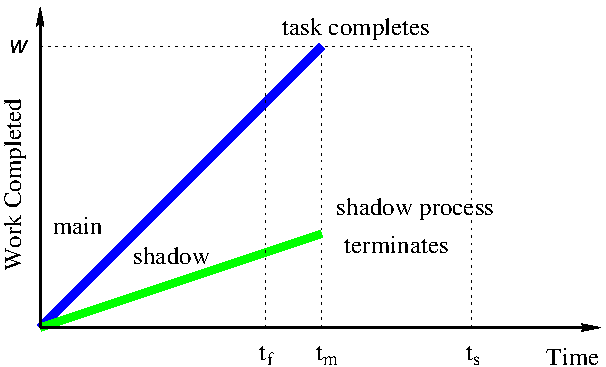
\includegraphics[width=0.7\columnwidth]{Figures/succ_new.pdf}
%		}
%		\subfigure[Main process failure.]
%		{
%			\label{fig:fail}
%			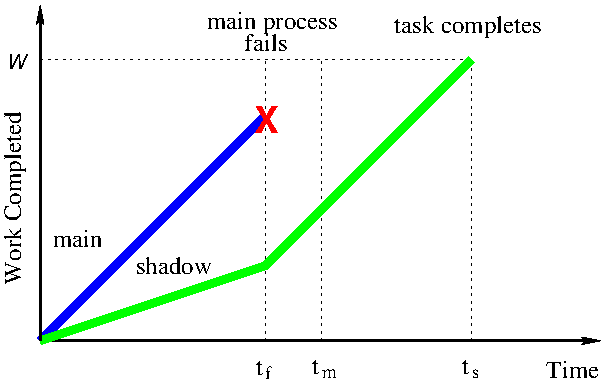
\includegraphics[width=0.7\columnwidth]{Figures/fail_new.pdf}
%		}
%	\end{center}
%	%\vskip -0.25in 
%	\caption{Lazy Shadowing execution dynamics.}
%	\label{fig:sync}
%\end{figure}

%The execution rate of the shadow before and , 

%For simplicity, we assume the maximum execution rate of a core is 1. 
In HPC, throughput consideration requires that the rate of the main, $\sigma_m$, and the rate of the shadow after failure, 
$\sigma_s^a$, be set to the maximum. 
The initial execution rate of the shadow, $\sigma_s^b$, however, can be derived by balancing the trade-offs between delay and energy.
%are determined based on the tolerance of the application to completion time.
For a delay-tolerant, energy-stringent application, $\sigma_s^b$ is set to 0, and the shadow starts executing only upon failure of the main process. %, for maximum energy saving. %, which guarantees additional energy is consumed only upon failure
For a delay-stringent, energy-tolerant application, the shadow starts executing at $\sigma_s^b=\sigma_m$ to guarantee the completion of the task at the specified time $t_m$, regardless of when the failure occurs. %In a word, Lazy Shadowing has the flexibility to converge to either rollback or process replication, if preferred,  
In addition, a broad spectrum of delay and energy trade-offs in between can be explored either empirically or by using optimization frameworks for delay and energy tolerant applications.
%For elastic applications, the delay-energy product can be used to derive the execution rate  
%For other applications, $\sigma_s^b$ and $\sigma_s^a$ can be derived by balancing trade-offs between completion time and energy consumption
%however, may still be tuned to manage the trade-offs between completion time and energy consumption. Smaller $\sigma_b$ corresponds to lazier shadowing of the main process.

 %Figure~\ref{fig:succ} illustrates the execution scenario with no failure, while Figure~\ref{fig:fail} depicts the scenario where the main process fails.




%In terms of execution rates, this can be expressed as $\sigma_m=\sigma_a=1$ and $\sigma_s \le 1$.  






\section{Extreme-scale fault tolerance}
\label{frame_multiple}
Enabling Lazy Shadowing for resiliency in extreme-scale computing 
brings about a number of challenges and design decisions that need to be addressed, including the applicability of this concept to a large number of 
tasks executing in parallel, the effective way to control shadows' execution rates, and the runtime mechanisms and 
communications support to ensure efficient coordination between a 
main and its shadow.
Taking into consideration the main characteristics of compute-intensive and highly-scalable applications, we design two novel techniques, referred to as {\it shadow collocation} and {\it shadow leaping}, in order to achieve high-tolerance to failure while minimizing delay and energy consumption. In the following, we first introduce the execution and communication model of the targeted applications. We then describe the dynamics of Lazy Shadowing with shadow collocation and shadow leaping. Lastly, we discuss important aspects of its implementation. 
%In the following, we first introduce the basic Lazy Shadowing resilience model. We then %focus on resilience in extreme-scale computing environments, where a large number of %communicating tasks execute in parallel to complete a job. 
%To achieve high tolerance to failure and reduce energy consumption in these environments, we %propose \emph{leaping shadows}, an instance of Lazy Shadowing. The main property of the %leaping shadows resilience model is its ability to sustain forward progress in the presence %of failures.
%. referred to as \emph{leaping shadows}, 
%a technique referred to as \emph{shadowed set rejuvenation} to reduce application failure probability, and 
%\emph{leaping shadows}, 
%as an 
%efficient, forward-progress preserving model to achieve high tolerance to failure, while reducing energy consumption, in these environments. 

 %We also discuss the runtime design issues
%related to enabling runtime support to efficiently achieve 
%the expected levels of resilience in extreme-scale systems. 

%This is to test referring Subsection \ref{frame_single}.



%\subsection{Application characteristics}
%\label{frame_app}
%%\subsection{Computational Model and Assumptions}
We consider the class of tightly-coupled and strongly scaled applications, executing on a large scale computing infrastructure of $N$ cores~\cite{doe_ascr_exascale_2011}. In this framework, the term core represents the unit of computing resource allocation (e.g., a
CPU core, a multi-core CPU, or a cluster node)~\cite{casanova_inria_2012}. This makes our framework agnostic to the granularity of the resource allocation unit.
%The focus of our model is a tightly-coupled and strongly scaling application, which executes on a large-scale platform
%composed of $N$ cores.
%We consider the execution of a tightly-coupled and strongly scaling application, or job, on a large-scale platform
%composed of $N$ cores. The application is tightly-coupled because this is typical in the HPC applications, and strong scaling because weak-scaling applications are not expected to suit for extreme-scale computing of which the cpu/memory imbalance would further increase~\cite{doe_ascr_exascale_2011}. Similar to \cite{casanova_inria_2012}, we use the term core to indicate unit of computing resource allocation (e.g., a
%CPU core, a multi-core CPU, or a cluster node), so that our work is agnostic to the granularity
%of the platform. 
%We assume that a standard checkpointing and roll-back recovery is performed at the
%system level. At most on application process (replica) runs on one core.


The application requires $W$ units of work, and can be split arbitrarily into a set of tasks.
Barriers are used as a method of synchronization among different tasks. Assuming $M \le N$ cores are assigned to the application, the failure-free completion time of the application is $w = W/M$. However, when a core fails, the whole execution will be suspended at the next barrier until recovery is complete. 

%The job can execute on any number $M \le N$ cores. The job is strong scaling so that the time required for a failure-free execution on $M$ cores is $w = W/M$.

%Cores are subject to failures. In most cases, we do not distinguish between soft and hard failures, with the understanding that soft failures are handled via software rejuvenation (i.e., rebooting \cite{466961}) and that hard failures are handled by the replacement of the failed component with a spare, which is a commonplace approach in production systems. For simplicity, we adopt the fail-stop fault model, where a core stops execution once a failure occurs and the failure can be detected by other cores \cite{gartner_faults_1999,cristian_comm_1991}. Since we consider tightly coupled parallel jobs, all $M$ cores operate synchronously. When a core fails, the whole execution is suspended until the failure is recovered. We assume that core failures are independent and identically distributed (i.i.d.). In the real world, instead, failures are bound to be correlated. Obtaining theoretical results for non-i.i.d. failures is beyond the scope of this work. But note that one cause of correlation is the hierarchical structure of computing platforms (each rack comprises compute nodes, each compute node comprises processors, and each processor comprises cores), which leads to simultaneous failures of a group of cores. Our work applies to such failures since a group of failures can be treated as multiple individual failures that happen at the same time and their recovery can be carried out in parallel.

Cores are subject to failures. In our model, we do not distinguish between soft and hard failures. We further assume that soft failures are handled via software rejuvenation (i.e., rebooting \cite{466961}), while hard failures are handled by replacing the failed components with spares. We adopt the fail-stop fault model, whereby a core stops executing upon failure and failures are detected by other non-failing cores \cite{gartner_faults_1999,cristian_comm_1991}. When a core fails, the whole execution is suspended until recovery is complete. 

%%%%%%%%%%%%%%%%%%%%%%%%%%%%%%rethinking%%%%%%%%%%%%%%%%%%%%%%
We assume that core failures are independent and identically distributed (i.i.d.). In the real world, instead, failures are bound to be correlated. Obtaining theoretical results for non-i.i.d. failures is beyond the scope of this work. But note that one cause of correlation is the hierarchical structure of computing platforms (each rack comprises compute nodes, each compute node comprises processors, and each processor comprises cores), which leads to simultaneous failures of a group of cores. Our work applies to such failures since a group of failures can be treated as multiple individual failures that happen at the same time and their recovery can be carried out in parallel.

%Since we consider tightly coupled parallel jobs, all q cores operate syn- chronously. These cores execute the same amount of work W(q) in parallel, chunk by chunk. The total time (on one core) to execute a chunk of dura- tion, or size, ω and then checkpointing it, is ω + C(q)

%\subsection{Leaping Shadows}



%%%%%%%%%%%%%%%%%%%%%%%%%%%%%%%%%%%%%%%%%%%%%%%%%%%%%%%%%%%%%%%%%%%%%%%%%%%%%%%%%%

%%We consider the class of strongly-scaled applications, and use $W$ to denote the size of an application workload~\cite{doe_ascr_exascale_2011}. The workload is split  arbitrarily into a set of $N$ tasks, whose synchronization is achieved using barriers. Assuming that each task is assigned to execute on a core at a maximum speed $\sigma=1$, the failure-free completion time of the application is $w = W/N$. 
Let $M_i$ denote the main process executing the $i^{th}$ task $T_i$, and $S_i$ its associated shadow.
When a failure occurs, the non-failing tasks continue executing until they reach the synchronization barrier. The tasks remain suspended until the shadow associated with the failing task reaches its synchronization barrier.


failure recovery is achieved.  To reduce time to recovery,  we run M shadows simulataneously with the main processes. 
%According to the computational model in Section~\ref{sec:com_model}, an application's workload is split into $M$ parallel tasks where each task is associated with a main process and a shadow.

 The execution of the application can be carried out by simultaneously running all main and shadow processes 
on %$2M$ cores, whereby the main processes execute at the maximum rate while the associated shadows execute at a fraction, $\sigma_s$, of the 
%maximum rate using DVFS. 
%To simultaneously run all the main and shadow processes,
%ne may choose to use $2M$ cores, with $M$ executing the main tasks at the maximum rate and $M$ \emph{lazily} executing the shadows at a fraction, $\sigma_s$, of the 
%maximum rate using DVFS.  
%An alternative method is to use 
$M+S$ cores, where $M$ is a multiple of $S$ and $M+S=N$, all executing at the maximum rate. $M$ of these cores are allocated to the main processes while the remaining $S$ cores are shared among their associated shadows. Based on this method, each main process is allocated one core, while $\alpha=M/S$ shadows are collocated on a single core. $\alpha$ is referred to as the main to shadow ratio.
For example, if $M=9$ and $S=3$, then the 9 shadows execute on 3 cores, with every $\alpha=3$ shadows executing on a core (Figure~\ref{fig:sc_mapping}).
%only $M+S$ cores can be used, whereby the main processes execute on the $M$ cores. And the $M$ shadows are divided into $S$ clusters with of $M/S$ shadows are colocated on a single core, operating at the maximum rate.
%where $M$ is a multiple of $S$, and collocate $M/S$ shadows on each of the $S$ cores, while executing all the cores at the maximum speed. 
%We use $\alpha$ to denote the main to shadow allocation ratio. %, and for simplicity, we assume the maximum execution rate of a core is 1. %Ignoring the overhead of context switching, the two alternatives lead to the same expected execution time, but different power and energy consumption. Specifically, the $2M$-cores scheme consumes more static but less dynamic power/energy than the $M+S$ cores alternative. The ratio between the system static and dynamic power consumption determines which alternative overall consumes less power/energy. 

%In the rest of the paper, we will focus on 
%shadow collocation as the meain the rest of our discussion 
%of the main ideas, concepts and system design. We will assume that all cores in the system execute at maximum speed, with every $\alpha=M/S$ shadows collocated on a core. 
%In HPC, throughput consideration requires that the rate of the main task, $\sigma_m$, and the shadow after failure, $\sigma_a$, be set to the maximum. The execution rate of the shadow before failure, $\sigma_b$, however, may still be used to manage the trade-offs between completion time and energy consumption. Smaller $\sigma_b$ corresponds to lazier shadowing of the main process. 
%In terms of execution rates, this can be expressed as $\sigma_m=\sigma_a=1$ and $\sigma_s \le 1$. 
  
Collocation of $\alpha$ shadows on a core has an important ramification with respect to the resilience of the system. Specifically, to speed up a shadow 
of a failed main to the maximum rate, all other collocated shadows must be terminated. Consequently, a second failure in any of the mains of the terminated shadows cannot be tolerated. In other words, the $M+S$ cores are grouped into $S$ sets, which we call \emph{shadowed sets}, each containing $\alpha+1$ cores with $\alpha$ mains executing on $\alpha$ cores (referred to as main cores) and their corresponding $\alpha$ shadows collocated on one core (referred to as shadow core). Each shadowed set can tolerate a failure in any of its cores, since failure of a main core would be recovered by the shadow core and failure of the shadow core will not affect any mains. After the first failure in a shadowed set, the set is called \emph{vulnerable} because it cannot tolerate another failure. %In the following subsection, we will discuss a rejuvenation scheme that deals with vulnerable shadowed sets.

\begin{figure}[!t]
	\begin{center}
		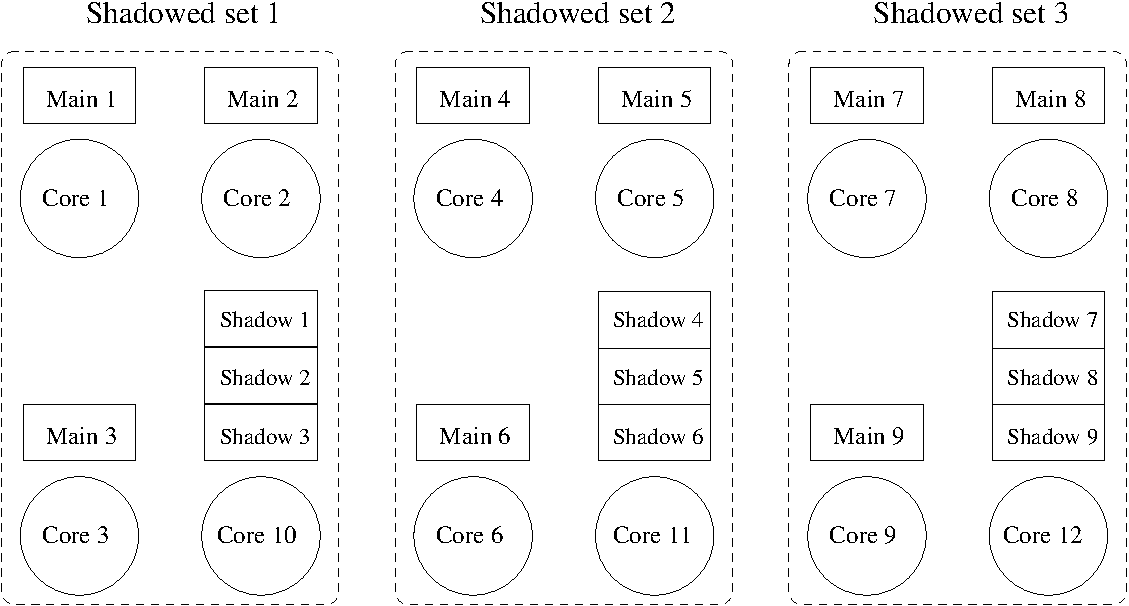
\includegraphics[width=\columnwidth]{Figures/sc_mapping.pdf}
	\end{center}
	\vskip -0.25in 
	\caption{An example of 3 shadowed sets with $\alpha=3$.}
	\label{fig:sc_mapping}
\end{figure}

%Lazy Shadowing provides the basis for the design of efficient energy- and power-aware fault-tolerance solutions for extreme-scale computing environments. %The resulting model, referred to as {\it leaping shadows}, 


%Lazy shadowing provides the basis for the design of efficient energy- and power-aware fault-tolerance solution for extreme-scale computing environments. The resulting model, referred to as {\it leaping shadows}, takes into consideration the main characteristics of compute-intensive and highly-scalable applications to achieve high-tolerance to failure, while minimizing energy consumption. In the following, we first introduce the execution and communication model of the targeted applications. We then describe the dynamics of the {\it leaping shadows} resilience model. Lastly, we discuss important aspects of its implementation. 
\subsection {Application model}
\label{sec:app_model}

We consider the class of compute-intensive and strongly-scaled applications, executing on a large-scale multi-core computing infrastructure~\cite{doe_ascr_exascale_2011}. %Communication between cores is achieved using low-latency, high-bandwidth interconnect networks, such as Infiniband. 
We use $W$ to denote the size of an application workload, and assume that the workload is split into a set of tasks, $T$, which execute in parallel. % and are synchronized using barriers. 
Assuming the maximum execution rate is $\sigma_{max}=1$, the failure-free completion time of the application is $W/|T|$. 
Given the prominence of MPI in HPC environments, we assume message passing as the communication mechanism between tasks. %Based on this model, each pair of communicating tasks is associated with a logical first-in-first-out (FIFO) channel, which guarantees ordered delivery of messages.
The execution is composed of a set of iterations separated by synchronization barriers. 
%The execution is divided into a set of phases by synchronization barriers. 


 %If a failure occurs, however, the non-failing tasks would become idle when they reach their synchronization barrier. These tasks remain idle until the failure recovery is complete. 
%resulting in performance hiccups~\cite{muller2010}, especially for tightly-coupled applications. 


\subsection{Shadow collocation}

%The execution of an application can be carried out by simultaneously running all tasks, each with a pair of main and shadow processes. Let $m_i$ denote the main process executing the $i^{th}$ task $\tau_i$, and $s_i$ its associated shadow.
%There are multiple ways to control the execution rates of the processes. The most straightforward solution is to allocate a dedicated core for each process while using 
%Dynamic Voltage and Frequency Scaling (DVFS) is a commonly used power management technique 
We use the term core to represent the resource allocation unit (e.g., a
CPU core, a multi-core CPU, or a cluster node), so that our algorithm is agnostic to the
granularity of the hardware platform~\cite{casanova_inria_2012}. Each main process executes on one core exclusively to achieve maximum throughput.  
To control the shadow's execution rate, Dynamic Voltage and Frequency Scaling (DVFS) can be applied while each shadow also uses one core exclusively~\cite{mills_2014_icnc,cui_en7085151,cui_2014_closer}. 
The effectiveness of DVFS, however, may be markedly 
limited by the granularity of voltage control, the number of frequencies available, and the negative effects on 
reliability~\cite{chandra2008defect}.
%reduced in computational platforms that exhibit saturation of the processor clock frequencies, large static power consumption, or small power dynamic range. 
 %Given our focus on extreme-scale, multi-core computing infrastructure, we will use collocation for execution rate control.  
%Recent development in processor and memory technology which results in the saturation of the processor clock frequencies, larger static power consumption, and smaller power dynamic range can markedly reduce the effectiveness of DVFS

 %to tune the frequency of the core. An alternative is to collocate multiple processes on a core, which runs at the maximum rate, and execute the processes in a time sharing manner. In the rest of this paper, we will focus on the idea of collocation in the discussion of applying Lazy Shadowing to HPC applications.  

An alternative is to collocate multiple shadows on a single core while keeping the core at maximum rate. Time sharing can then be used to achieve the desired execution rates.
To execute an application of $M$ tasks, $N=M+S$ cores are required, where $M$ is a multiple of $S$. Each main is allocated one core (referred to as \textit{main core}), while $\alpha=M/S$ (referred to as \textit{collocation ratio}) shadows are collocated on a core (\textit{shadow core}). 
The $N$ cores are grouped into $S$ sets, each of which we call a \textit{shadowed set}. Each shadowed set contains $\alpha$ main cores and 1 shadow core.
% $\alpha$ is referred to as shadowing ratio. For example, if $M=9$ and $S=3$, then the 9 shadows share 3 cores, with every $\alpha=3$ shadows collocated on each core, as shown in Figure~\ref{fig:sc_mapping}.
This is illustrated in Figure~\ref{fig:sc_mapping}.  

Collocation has an important ramification with respect to the resilience of the system. Specifically, 
one failure can be tolerated in each shadowed set. If a shadow core fails, all the shadows in the 
shadowed set will be lost without interrupting the execution of the mains. 
On the other hand, if a main core fails, the associated shadow will be promoted to a new main, and all 
the other collocated shadows will be terminated to speed up the new main.
%to speed up a shadow 
%of a failed main to the maximum rate, all other collocated shadows must be terminated. 
Consequently, a failure, either in main or shadow core, will result in losing all the shadows in the shadowed set, thereby losing the tolerance to any other failures. %After the first failure, a shadowed set becomes \emph{vulnerable}\footnote{Rejuvenation techniques, such as restarting the lost shadows from the state of current mains on spare cores, can be used to eliminate vulnerability.}. 
Quantitative study of this effect using probability theory is presented in Section~\ref{anal_app_fail}. %, this should not be a concern as the provided reliability is more than enough.
 
\begin{figure}[!t]
  \begin{center}
    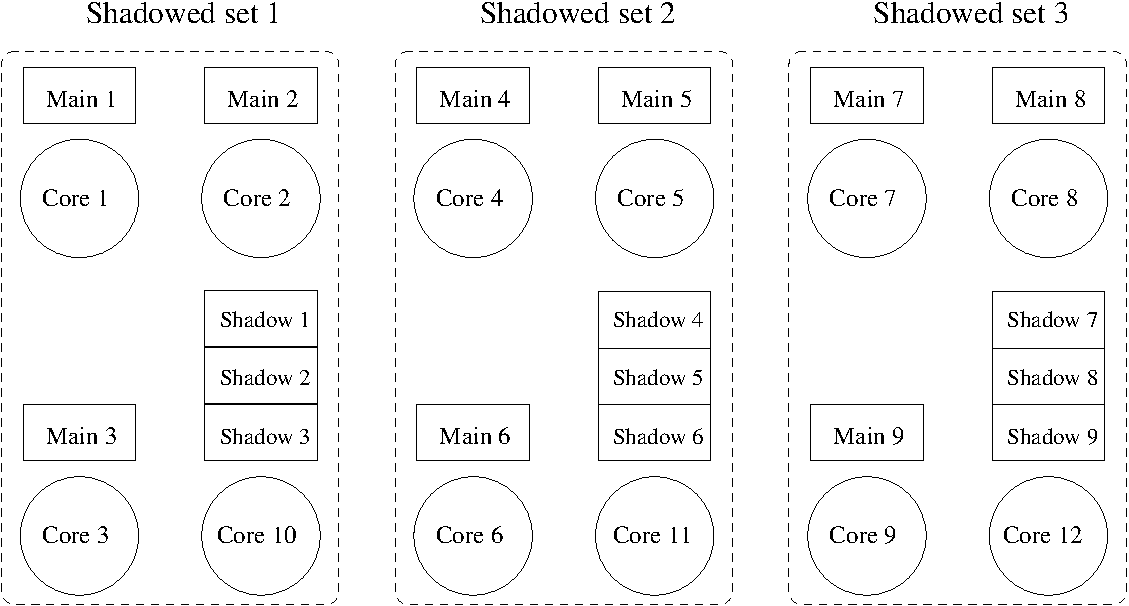
\includegraphics[width=\columnwidth]{Figures/sc_mapping.pdf}
  \end{center}
  %\vskip -0.25in 
  \caption{An example of collocation. $N=12$, $M=9$, $S=3$.}
  \label{fig:sc_mapping}
\end{figure}




\subsection {Shadow leaping}
\label{sec:leaping_shadows}

As the shadows execute at a lower rate, failures will incur delay for recovery. This problem deteriorates as dependencies incurred by messages and synchronization barriers would propagate the delay of one task to others.  
%The main objective of shadow leaping shadows is to minimize the delay induced by failures, 
%mitigate the impact of performance hiccups, 
Fortunately, slowing down the shadows provides an opportunity for the shadows to benefit from the faster execution of their mains. By copying the state of each main to its shadow, which is similar to the process of storing a checkpoint in a buddy in \cite{zheng_2004_ftccharm}, forward progress is achieved for the shadows with minimized time and energy. This technique, referred to as \textit{shadow leaping}, effectively limits the distance between main and shadow in progress. 
%, which simultaneously reduces the recovery time for failures. 
As a result, the recovery time after a failure, which depends on the distance between the failing main 
and its shadow, is also reduced. 
More importantly, %shadow leaping does not necessarily require the stopping of all the mains during normal execution, which will incur extra overhead even for failure-free execution. 
%Instead, 
we opportunistically overlap shadow leaping with failure recovery to avoid extra overhead. 
%and ensure forward progress by opportunistically rolling-forward the shadows during failure recovery. In Section~\ref{anal_time}, we will show that the delay is well bounded even for tightly-coupled applications.

%In the absence of failure, the behavior of a main  and its leaping shadow is identical to the behavior depicted in Figure \ref{fig:sync}. 
Assuming a failure occurrence at time $t_f$, Figure~\ref{fig:leap} shows the concept of shadow leaping. 
%Figure~\ref{fig:jump1} depicts the execution dynamics of the failing main and its associated shadow. 
Upon failure of a main process, its associated shadow speeds up to minimize the impact of failure recovery on the other tasks' progress, as illustrated in Figure~\ref{fig:jump1}. 
%Figure~\ref{fig:jump2} illustrates the behavior of the remaining main processes and their associated shadows. 
At the same time, as shown in Figure~\ref{fig:jump2}, the remaining main processes continue execution until the barrier at $W_{syn}$, and then become idle until $t_r$. %, when the shadow of the failed main also reaches the barrier. %It is worth noting that, given the tightly-coupled and strongly-scaled nature of the application, synchronization points occur frequently. Consequently, the time between synchronization points is very small relative to the total execution time of the application. Therefore, if one main, $m_i$, fails at 
%time $t_f$, the remaining main processes will reach their synchronization point, shortly after the failure, specifically at at time $t_{sync} = t_f +\epsilon$, 
%where $\epsilon \approxeq 0$. 
Shadow leaping opportunistically takes advantage of this idle time to {\it leap forward} the shadows by copying state from their mains, so that  
all processes, including shadows, can resume execution from a consistent point afterwards. %This process continues until the completion of all tasks. 
Shadow leaping increases the shadow's rate of progress, at a minimal energy cost. Consequently, it reduces significantly the likelihood of a shadow falling excessively behind, thereby ensuring fast recovery while minimizing energy consumption.



\begin{figure}[!t]
	\begin{center}
        \subfigure[Faulty task behavior.]
		{
			\label{fig:jump1}
			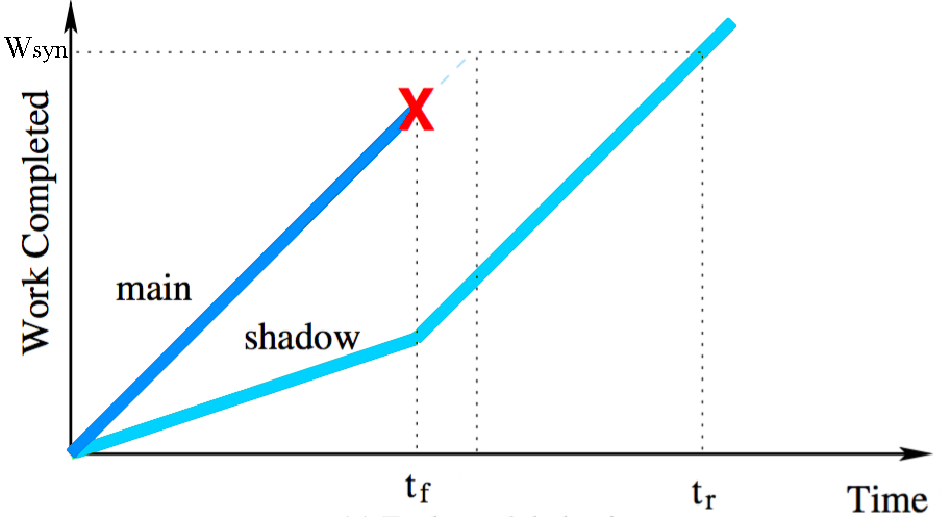
\includegraphics[width=0.7\columnwidth]{Figures/jump1.pdf}
		}
		\subfigure[Non-faulty task behavior.]
		{
			\label{fig:jump2}
			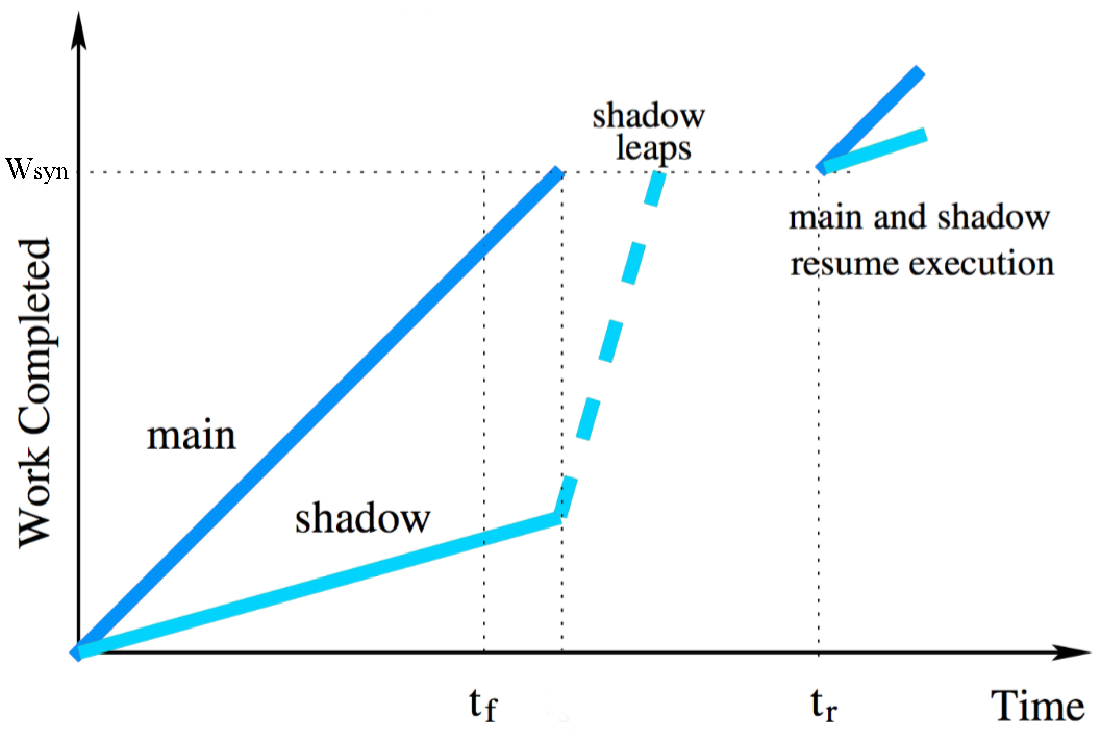
\includegraphics[width=0.7\columnwidth]{Figures/jump2.pdf}
		}
	\end{center}
	%\vskip -0.25in
	\caption{The illustration of shadow leaping.}
	\label{fig:leap}
\end{figure}

%Collocation is used to control the execution rates. To execute an application with $M$ tasks, $N=M+S$ cores are required, where $M$ is a multiple of $S$. Each main process is allocated one core (referred to as main core), while $\alpha=M/S$ shadows are collocated on a core (shadow core). 
%The $N$ cores are grouped into $S$ sets, which we call \emph{shadowed sets}, each containing $\alpha$ main cores and 1 shadow core.
%% $\alpha$ is referred to as shadowing ratio. For example, if $M=9$ and $S=3$, then the 9 shadows share 3 cores, with every $\alpha=3$ shadows collocated on each core, as shown in Figure~\ref{fig:sc_mapping}.
%This is illustrated in Figure~\ref{fig:sc_mapping}.  
%Collocation has an important ramification with respect to the resilience of the system. Specifically, 
%one failure can be tolerated in each shadowed set. If a shadow core fails, the main processes can continue
%execution, but will have no shadows any more. On the other hand, 
%to speed up a shadow 
%of a failed main to the maximum rate, all other collocated shadows must be terminated. Consequently, a second failure in any of the mains in the shadowed set cannot be tolerated. After the first failure, a shadowed set becomes \emph{vulnerable}\footnote{Rejuvenation techniques, such as restarting the lost shadows from the state of current mains on spare cores, can be used to eliminate vulnerability.}. 
%
%\begin{figure}[!t]
%  \begin{center}
%    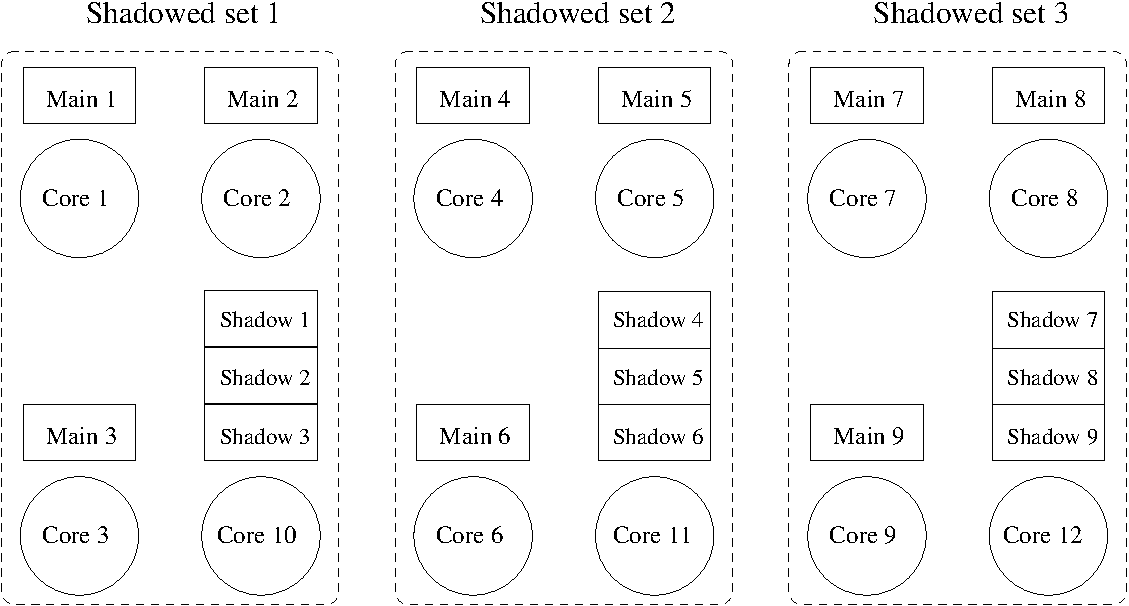
\includegraphics[width=\columnwidth]{Figures/sc_mapping.pdf}
%  \end{center}
%  %\vskip -0.25in 
%  \caption{An example of collocation. $N=12$, $M=9$, $S=3$.}
%  \label{fig:sc_mapping}
%\end{figure}

%Collocation also increases memory requirement. However, this is not intrinsic to Lazy Shadowing, as checkpointing/restart also requires additional memory capacity. We acknowledge the fact that compute kernels in existing HPC environments were simplified significantly by placing a number of restrictions, including eliminating virtual paging and limiting support for OS (Linux) to a handful of system calls. It became clear, however, that strategies designed to work around the capabilities of the hardware cannot scale to extreme-scale computing. Consequently, the research focus has been on new paradigms focused on co-design of hardware with system software to leverage the advantages associated with dynamic, asynchronous mechanisms, such as demand paging and cache tuning, against the design principles and choices of current HPC systems. Support of efficient demand paging, through co-design, is particularly critical as it is expected that the data of future exascale applications may not fit entirely in memory. %Finally, in comparison to checkpointing/restart and process replication, Lazy Shadowiing has the capability to control memory usage, based on the nature of failure and existing memory capacity, albeit at a loss of performance. 



\begin{algorithm}[t]
  \SetKwInOut{Input}{input}
  \SetKwInOut{Output}{output}
  \caption{Lazy Shadowing}
  %\Input{$W, M, S$}
  \Input{$M, S$}
  \Output{Application execution status}
  \BlankLine
  %split $W$ into $M$ tasks\; \nllabel{line:split} 
  %assign $M$ tasks to $S$ shadowed sets\; \nllabel{line:cluster} 
  %$T_l \leftarrow T+t_{now}$\;%, $C_{vul} \gets 0$
  %start $m_i$ and $s_i$ for each $task_i$\;
  start $M$ pairs of main and shadow\;
  map processes to cores\;
    \While{execution not done}
    {
  %      \If{failure detected in $ss_j$} %\nllabel{line:if_start_1} 
        \If{failure detected}
        {
            \nllabel{line:if_start_1} 
            %\eIf{$ss_j$ is vulnerable}
            \eIf{shadowed set is vulnerable}
            {
                notify ``Application fatal failure"\;
                %terminate all mains and shadows\;
                %repair all failures\;
                restart execution\; %\Comment{re-execution}
            }
            {
                mark the shadowed set as vulnerable\;
                %\State $C_{vul} \gets C_{vul} + 1$
                %\If{$C_{vul} == V$}
                %    \State perform shadowed set rejuvenation   
                %\EndIf 
                \If{failure happened to a main} 
                {
                    promote its shadow to new main\;
                    triggers shadow leaping\; %failure induced shadow leaping
                    %$T_l \leftarrow T+t_{now}$\;
                }
            }
        }  
        \nllabel{line:if_end_1}
        %\If{$t_{now} \ge T_l$} %
        %{
        %    \nllabel{line:if_start_2} 
        %    perform shadow leaping\;
        %    $T_l \leftarrow T+t_{now}$\;
        %    \nllabel{line:if_end_2}
        %} % 
        %\nllabel{line:if_end_2}
    }
    output ``Application completes"\;
  \label{al:ls}
\end{algorithm}

%The steps of applying Lazy Shadowing with leaping shadows are depicted in Algorithm 1.
We summarize the integration of shadow collocation and shadow leaping with basic shadowing in Algorithm 1.
User needs to specify $M$ for the number of parallel tasks, and $S$ for the number of shadow cores. These two parameters jointly determine the collocation ratio $\alpha=M/S$. The execution starts by simultaneously launching $2M$ processes, of which one main is associated with one shadow for each task (line 1). 
All processes are then grouped into $S$ shadowed sets. Accordingly, the processes are mapped to cores so that each shadowed set has $\alpha$ cores for $\alpha$ mains and 1 core for all the associated shadows (line 2). 
%To use $M+S$ cores to execute an application, the total workload is split into $M$ parallel tasks (line~\ref{line:split}), %, which are executed simultaneously by $M$ main processes and $M$ shadow processes. 
% which are then assigned to $S$ shadowed sets, each with $\alpha=M/S$ cores for $\alpha$ main processes and 1 core for all the associated shadow processes (line 2).  
%The $M$ shadows are then clustered into $S$ groups, each containing $\alpha=M/S$ shadows. 
%The execution starts by simultaneously running all the main and shadow processes (line 3).
During the execution,
the system runs a failure monitor (e.g., by using heartbeat protocol~\cite{1004595}) that triggers corresponding actions when a failure is detected (line~\ref{line:if_start_1} to~\ref{line:if_end_1}). %A failure may trigger different actions, depending on its type and precedence with respect to other failures.  A shadowed set becomes {\it vulnerable} after the occurrence of the first failure in the set. 
A failure occurring in a vulnerable shadowed set results in an application fatal failure %. In response, the system terminates all running 
%processes, initiates a recovery phase, either by rebooting or replacing failing cores,  and restarts execution (line 8 to 10). %(this assumes that checkpointing is not used). 
 and forces a rollback (line 6 and 7).
On the other hand, failure in a non-vulnerable shadowed set
can be tolerated while making the target shadowed set vulnerable (line 9). In this case, failure of a main need to be treated differently from failure of a shadow. While a failure of shadow 
does not impact the normal execution and thus can be ignored, failure of a main %forces the remaining main processes to suspend execution after they reach their synchronization point.  The shadow process, $s_k$, associated with the failing process, $m_k$,  becomes the primary process of the associated task and increases its execution to the maximum rate 
triggers promotion of its shadow to a new main, which increases its rate to recover the failure and complete the task (line 11). Simultaneously, a shadow leaping is undertaken by all other shadows to align their states with those of their associated mains (line 12).  
This process continues until all tasks of the application are successfully completed.

\subsection{Implementation issues}

%\subsection{Shadowed set rejuvenation}
%\label{frame_reju}
%The proposed Lazy Shadowing scheme can tolerate faults which are repairable by rebooting or reconfiguration, referred to as soft faults, and faults which cannot be repaired by rebooting or reconfiguration, referred to as hard 
faults. Monitors that detect hard faults, such as memory flip, bus error 
and latch error, or soft faults, such as deadlock detection, buffer overflow and protection violation, typically interrupt the application to initiate 
the recovery process. The process of recovery from transient or permanent faults is the same and necessitates a mechanism for detecting a fault 
in a main task, M(i) and notifying other tasks in the system so that (i) the shadows sharing a core with S(i) are terminated, thus allowing S(i) to execute at the maximum rate, and (ii) all the shadows that are not in the faulty shadowed set leap to the state of their mains. 

As described earlier, the recovery from a fault in a shadowed set leaves the set vulnerable and any more faults in a vulnerable set will result in a system failure. Although for large systems and small S the probability of having a second fault in a vulnerable set is low, some provision should be taken to rejuvenate the system when a relatively large number of its shadowed sets are vulnerable. 

We propose to invoke \emph{shadowed set rejuvenation} after a specific number of faults, which is determined by the system size, the shadowed set size, and the required resilience.
Rejuvenation reconfigures the system such that none of its shadowed sets are vulnerable. Unlike recovery from a fault in a shadowed set, rejuvenation is different when the faults are transient soft when the faults are hard. In the case of soft faults, rejuvenation can be accomplished by rebooting the failed cores, and restarting the lost shadows (both the ones promoted to mains and the ones terminated) from the state of current mains. And in case of hard faults, it is possible to restart the lost shadows after replacing the failed ones with spare ones. This will restore a vulnerable shadowed set to its original configuration. %For example, rejuvenation should restore the systems shown in Figure~\ref{fig:layout2} and Figure~\ref{fig:layout3} to the one shown in Figure~\ref{fig:layout1}.

%When failures are permanent, rejuvenation may be challenging if rebooting or reconfiguration can no longer be
%used to recover failed components.
%Specifically, in the absence of spare components (if the system is not over-provisioned),
%rejuvenation can only 
%be accomplished by distributing the main processes of a vulnerable set 
%to other {\bf non-vulnerable} shadowed sets. The shadow of the vulnerable 
%set must also be relocated to the shadows of the non-vulnerable set. 
%As a result,  the total number of shadowed sets decreases, but 
%the size of some shadowed sets increases.  In Figure~\ref{fig:reju}, we show a possible rejuvenated configuration assuming that the failure of the cores executing $M(1)$ and $M(14)$ in Figure~\ref{fig:layout2} is permanent. In this restored configuration, the number of shadowed sets is reduced from 8 to 6, with four sets containing three mains each and two sets containing two mains each. Rejuvenating the vulnerable configuration of Figure~\ref{fig:layout3} after a permanent socket failure is more complex but follows the same basic principle.

%\begin{figure*}[ht]
%	\begin{center}
%		\includegraphics[width=\textwidth]{figures/reju.pdf}
%	\end{center}
%\vskip -0.25in
%	\caption{Shadowed set rejuvenation of the vulnerable sets resulting from permanent faults.}
%	\label{fig:reju}
%\end{figure*}


%%%%%%%%%%%%%%%%%%%%%%%%%%%%%%%%%%%%%%%%%%%%%%%%%%%%%%%%%%%%%%%%%%%%%%%%%%%%%%%%%%
%We implemented an Open MPI based prototype of Lazy Shadowing, which can be used to execute existing HPC workloads without any change of user code. 
We are implementing a MPI based library for Lazy Shadowing, referred to as lsMPI. Inserted as a layer between application and MPI, lsMPI uses the MPI profiling hooks to intercept every MPI call. Currently, lsMPI 
delegates failure detection to ULFM, which guarantees that an error code is returned if failure prevents 
an MPI operation from completion
~\cite{Bland:2012:EUF:2404033.2404064,bland2013post}. 
lsMPI should be portable across all MPI implementations once extensions by ULFM are added to MPI standard.
%Since the focus of this paper is to introduce
%algorithmic perspectives of the Lazy Shadowing paradigm by discussing novel concepts of shadow collocation and shadow leaping, we only give a brief discussion of the implementation issues. 

State consistency is required both during normal execution and following a failure. % of a main process to roll-forward the shadows. 
We design a consistency protocol %in Figure~\ref{fig:cons_protocol}
to assure 
that the shadows see the same message order and MPI results as mains. %In this figure, A and B represent two mains, and A' and B' are their shadows. 
For each message, the main sender sends a copy of the message to each of the main and shadow receivers. After getting the message, the main receiver sends an ACK to the shadow sender, so that the shadow sender can safely suppress sending the message and proceed. If a main fails,
its associated shadow will become a new main and start sending out messages. The ACK messages, plus one NAK message after the failure, guarantee that the new main is always consistent with the other mains. 
%We bare the risk of temporarily losing consistency between the new main and the shadow receiver, 
Although the remaining shadows may temporarily be inconsistent with the new main after the failure, shadow leaping will bring them back to a consistent state.
%Since MPI implements reliable network transportation, the shadow receiver will eventually get the same message as its main, unless a failure occurs. We don't require the shadow receiver to sends ACK to the shadow sender during normal execution. If the main sender fails, the shadow sender will become a new main and start sending out messages. To avoid duplicate messages, the main receiver will use a NAK message to tell the new main the next message it needs. Since previously we require the shadow sender to get an ACK before suppressing a message, the shadow sender will never suppress a message that the main receiver would need, even in the cases of failure. Without using ACK, the shadow receiver may become inconsistent with the new main. However, by aligning the state of the shadow receiver with that of its main we assure that the shadow receiver will be in a consistent state after shadow leaping. 

%\begin{figure}[!t]
%  \begin{center}
%      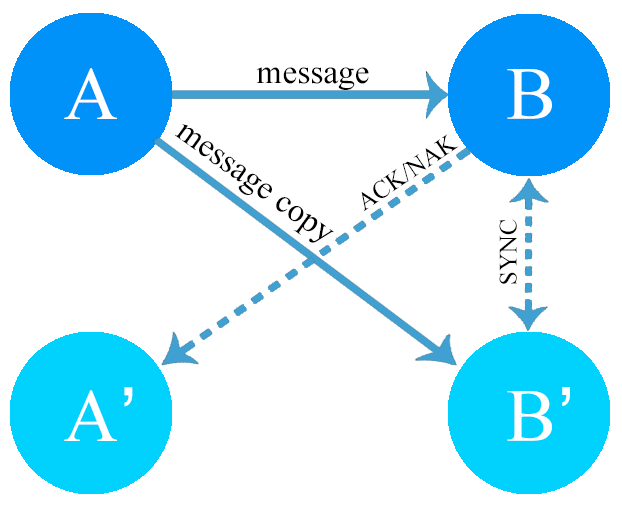
\includegraphics[width=0.7\columnwidth]{Figures/cons_protocol}
%  \end{center}
%  %\vskip -0.25in
%  \caption{Consistency protocol for lsMPI.}
%  \label{fig:cons_protocol}
%\end{figure}

We assume that only MPI operations can introduce non-determinism. MPI\_ANY\_SOURCE receives may result in different message orders between the main and shadow. To deal with this, we always let the main receive a message ahead of the shadow and then forward the message source to its shadow. %(SYNC message in Figure~\ref{fig:cons_protocol}). 
The shadow then issues a receive with the specific source. Other operations, such as MPI\_Wtime() and MPI\_Probe(), can be dealt with by always forwarding the result from the main to the shadow.

%Same as \cite{engelmann2011redundant,ferreira_sc_2011}, consistency protocol introduces runtime overhead due to extra messages. The overhead has been experimentally evaluated to be negligible for most real large-scale applications. Therefore, we believe our protocol, which reduces both message count and bandwidth requirement, should be acceptable. Currently, collectives in lsMPI use linear point-to-point operations internal to lsMPI. We plan to optimize its performance by using binomial tree topology and multi-level hierarchical topology considering hardware locality~\cite{herault2015practical}.

%During normal execution, shadows remain mute, in the sense that 
%all outgoing messages from shadows are suppressed. 
%A shadow process, however, will typically lag behind its main process during execution. Therefore, it is necessary to ensure that the shadow's state is consistent with that of its associated main. %, to successfully complete its associated task in case of failure. 
%To this end, a message-logging protocol is used, % to ensure consistency~\cite{Marz}. These protocols 
%which typically uses a minimum amount of meta-information to store and replicate the non-deterministic decisions~\cite{Marz}. %in the execution of an application.  These meta-data, also called determinants, are exchanged through system-level messages. 

%To provide correct recovery after failure, 
%a mechanism is required to guarantee that every shadow process follows the same computation and communication steps as its main process. 
%After a main fails, its associated shadow will become a new main to recover from this failure. If there are other shadows sharing the same core, they will be terminated and the new main will start consuming the messages in its receiver-side message log at a faster speed. The message logging protocol will ensure that after recovery the new main reaches a consistent state with the rest of the system. 

%Upon failure of a main process, shadow processes will update their address space to ``catch up" with their associated non-failing main processes. A technology, such as remote direct memory access (RDMA), can be used to roll-forward the state of the shadow to be consistent with that of its associated main. Rather than copying data to the buffers of the operating system, RDMA allows to transfer data directly from the main process to its shadow. The zero-copy feature of RDMA considerably reduces latency, thereby enabling fast transfer of data between the main and its shadow.

%Remote Direct Memory Access (RDMA) is used to leap forward the state of the shadow to be consistent with that of its associated main. Rather than copying data to the buffers of the OS, RDMA allows to transfer data directly from the main process to its shadow. The zero-copy feature of RDMA considerably reduces latency, thereby enabling fast transfer of data between the main and its shadow.

 




\section{\uppercase{Analytical Models}}
\label{sec:analytical}
Three important metrics for assessing the quality of an application's execution are 1) reliability; 2) completion time; and 3) energy consumption. In the following we develop mathematical models to analyze the expected performance of Lazy Shadowing, as well as prove the bound on performance compared to non-failure case, with the understanding
that process replication is a special case of Lazy Shadowing where $\alpha=1$. 
All the analysis below is under the assumption that there are a total of $N$ cores, and $W$ is the application workload.  
$M$ of the $N$ cores are allocated for main processes, each having a workload of $w=\frac{W}{M}$, and the rest $S$ cores are for collocated shadow processes. For process replication,
$M=S=\frac{N}{2}$, and $w=\frac{2W}{N}$. 


\subsection{Application fatal failure probability}
\label{anal_app_fail}
An application has to start over when one of its tasks has permanently lost its work. We call this an application failure, which is inevitable even when every process is replicated. Lazy Shadowing is able to 
tolerate one failure in each shadowed set. %, and the second failure in any shadowed set implies the need to restarting the execution from the very beginning. 
However, Lazy Shadowing is orthogonal to checkpointing in 
the sense that we can combine the two, to avoid rolling the execution back to the very beginning. 

Since each process is replicated with a shadow, Lazy Shadowing has the potential to significantly 
increase the Mean Number of Failures To Interrupt (MNFTI). % and Mean Time To Interrupt (MTTI).
%Therefore, the checkpointing interval should be increased to a large extent when checkpointing is combined with Lazy Shadowing. Furthermore, if the resulted checkpointing interval is 
%larger than the completion time of the application, then checkpointing may not be used at
%all. 
%Therefore, in this subsection, we study the reliability benefits that Lazy Shadowing could 
%introduce. Specifically, we study the application's MNFTI (and MTTI) with Lazy Shadowing.
%In the following, the first question to study is the new MNFTI and MTTI when Lazy Shadowing is used. 
The impact of process replication on MNFTI has been studied in~\cite{casanova_inria_2012}. %Our problem
%is equivalent to that, with the difference that our work can tolerate one failure in each shadowed 
%set while~\cite{casanova_inria_2012} can tolerate one failure in each replica-group of size 2. 
Applying the same methodology, we can derive the new MNFTI
with Lazy Shadowing for different number of shadowed sets ($S$), as shown in Table~\ref{tbl:mnfti}. 
%The MTTI with Lazy Shadowing is not shown here because it depends not only on the number of cores, but also on the shadowed set size chosen. However, results in \cite{casanova_inria_2012} reflect that the MTTI can be increased to the order of tens of hours from ten minutes (without use of replication) assuming the core level MTTI is 25 years. This 
%confirms our previous prediction that Lazy Shadowing can significantly 
%increase the application's MNFTI and MTTI, and also implies that shadowed set rejuvenation may not be necessary.
Note that when processes are not replicated, every failure would interrupt the application, i.e., MNFTI=1, so MNFTI can be significantly increased by Lazy Shadowing. 
It is projected that the Mean Time To Interrupt (MTTI) of an extreme-scale application can be increased to tens of hours from minutes assuming each core's MTBF is 25 years.
%\begin{table}[b!]
%	\caption{Application's MNFTI when Lazy Shadowing is used. Results are independent of $\alpha$. }
%	\centering
%	\small
%	\begin{tabular}{|c|c|c|c|c|c|c|c|}
%		\hline
%		$S$ & $2^{0}$ & $2^{1}$ & $2^{2}$ & $2^{3}$ & $2^{4}$ & $2^{5}$ & $2^{6}$ \\
%		\hline
%		MNFTI & 3.0 & 3.7 & 4.7 & 6.1 & 8.1 & 11.1 & 15.2\\
%		\hline\hline
%		$S$ & $2^{7}$ & $2^{8}$ & $2^{9}$ & $2^{10}$ & $2^{11}$ & $2^{12}$ & $2^{13}$ \\
%		\hline
%		MNFTI & 21.1 & 29.4 & 41.1 & 57.7 & 81.2 & 114.4 & 161.4 \\
%		\hline\hline
%		$S$ & $2^{14}$ & $2^{15}$ & $2^{16}$ & $2^{17}$ & $2^{18}$ & $2^{19}$ & $2^{20}$ \\
%		\hline
%		MNFTI & 227.9 & 321.8 & 454.7 & 642.7 & 908.5 & 1284.4 & 1816.0 \\
%		\hline
%	\end{tabular}
%	\label{tbl:mnfti}
%\end{table}


\begin{table}[b!]
	\caption{Application's MNFTI when Lazy Shadowing is used. Results are independent of $\alpha=\frac{M}{S}$. }
	\centering
	\small
	\begin{tabular*}{\columnwidth}{|c @{\extracolsep{\fill}} |c|c|c|c|c|}
		\hline
		$S$ &  $2^{2}$ &  $2^{4}$ &  $2^{6}$ & $2^8$ & $2^{10}$ \\ 
		\hline
		MNFTI &  4.7 & 8.1 & 15.2 & 29.4 & 57.7 \\
		\hline\hline
		$S$ & $2^{12}$ & $2^{14}$ &  $2^{16}$  & $2^{18}$ & $2^{20}$ \\
		\hline
		MNFTI & 114.4 & 227.9 & 454.7 & 908.5  & 1816.0 \\
		\hline
	\end{tabular*}
	\label{tbl:mnfti}
\end{table}


%Even though the above results imply that checkpointing may not be necessary when Lazy Shadowing is used, it is important to quantify the probability that an application failure would occur during the application's execution, defined as ``application failure probability". 
The level of reliability can be quantified by calculating the probability of application failure.
Let $f(t)$ denotes the failure probability density function of each core, then $F(t) = \int_0^tf(\tau)d\tau$ is the probability that a core fails in the next $t$ time. 
Since each shadowed set can tolerate one failure, 
then the probability that a shadowed set with $\alpha$ main cores and 1 shadow core does not fail by time $t$ is the probability of no failure plus the probability of one failure, i.e., 
%\begin{equation}
%	G(t, \alpha) = \Big(1-F(t)\Big)^{\alpha+1} + {{\alpha+1} \choose 1}F(t)\times \Big(1-F(t)\Big)^{\alpha}
%\end{equation}
\begin{equation}
	P_g = \Big(1-F(t)\Big)^{\alpha+1} + {{\alpha+1} \choose 1}F(t)\times \Big(1-F(t)\Big)^{\alpha}
\end{equation}
and the probability that the application using $N$ cores fails within $t$ time is the complement of the probability that
none of the shadowed sets fails, i.e.,
%\begin{equation}
%	R(t, N, \alpha) = 1 - \Big(G(t, \alpha)\Big)^{\frac{N}{\alpha+1}}
%\end{equation}
\begin{equation}
	P_a = 1 - ({P_g})^{S}
\end{equation}
where $S=\frac{N}{\alpha+1}$ is the number of shadowed sets.
The application failure probability can then be calculated by using $t$ equal to the expected completion time of the application, which will be modeled in the next subsection.
%that $T_c$ is a function of $W$, $N$, $\alpha$. As a result, the application failure probability can be expressed as $R'(W, N, \alpha)$.

%With $R(W, N, \lambda, S)$, we can study the behavior of lazy shadowing under a configuration of ($W$, $N$, application failure probability), for any failure distribution $f(t)$, e.g., exponential or weibull. However, there are two problems now: 1) The computation involved is so complicated that MatLab cannot give accurate results; 2) we don't have the analytical model of expected completion time $T_c$ assuming exponential or weibull failure distribution. 


\subsection{Expected completion time}
\label{anal_time}
One of the major performance metrics of interest to end-users, is the application's completion time. 
To evaluate this, we develop an analytical model for the expected completion time of Lazy Shadowing, with all probabilities of failures considered. For simplicity, we assume that no subsequent failure happens before the recovery of the previous failure. 
%Since we are comparing between Lazy Shadowing and process replication, the overhead of failure detection and consistency protocols are ignored as they are the same for the two approaches.
%Our models focus on one 
%checkpointing interval of the application, since the whole execution is just a repetition of multiple such intervals. As a consequence, we assume the execution with checkpointing starts right after the previous checkpoint and ends right before the next checkpoint, and the execution with Lazy Shadowing and process replication will not experience any application failure. For fairness, we assume that the three alternatives have the same amount of workload, 
%$W$, to execute, and total number of available cores, $M$. The maximal execution rate at each core, $\sigma_{max}$, is normalized to 1 so that the time to complete without failures is equal to the workload to execute on each core. In addition, we assume that the three alternatives will encounter the same number of failures, which is $k$, as they will execute the same amount of workload using the same amount of resources.

%\subsubsection{Expected completion time}
First we discuss the case of $k$ failures, which separate the execution into $k+1$ intervals. 
Denote by $\Delta_i$ ($1\le i \le k+1$) the $i^{th}$ continuous execution interval, and $\tau_i$ ($1\le i \le k$) the recovery time after $\Delta_i$. 
%between the $(i-1)^{th}$ and $i^{th}$ failures (assuming the $0^{th}$ failure happens right before the execution begins, and the $(k+1)^{th}$ failure happens right after the execution ends), and $\tau_i$ ($1\le i \le k$) the recovery time after the $i^{th}$ failure. 
The application's progress with delay incurred by failures is illustrated in Figure~\ref{fig:progress}.

\begin{figure}[!t]
	\begin{center}
		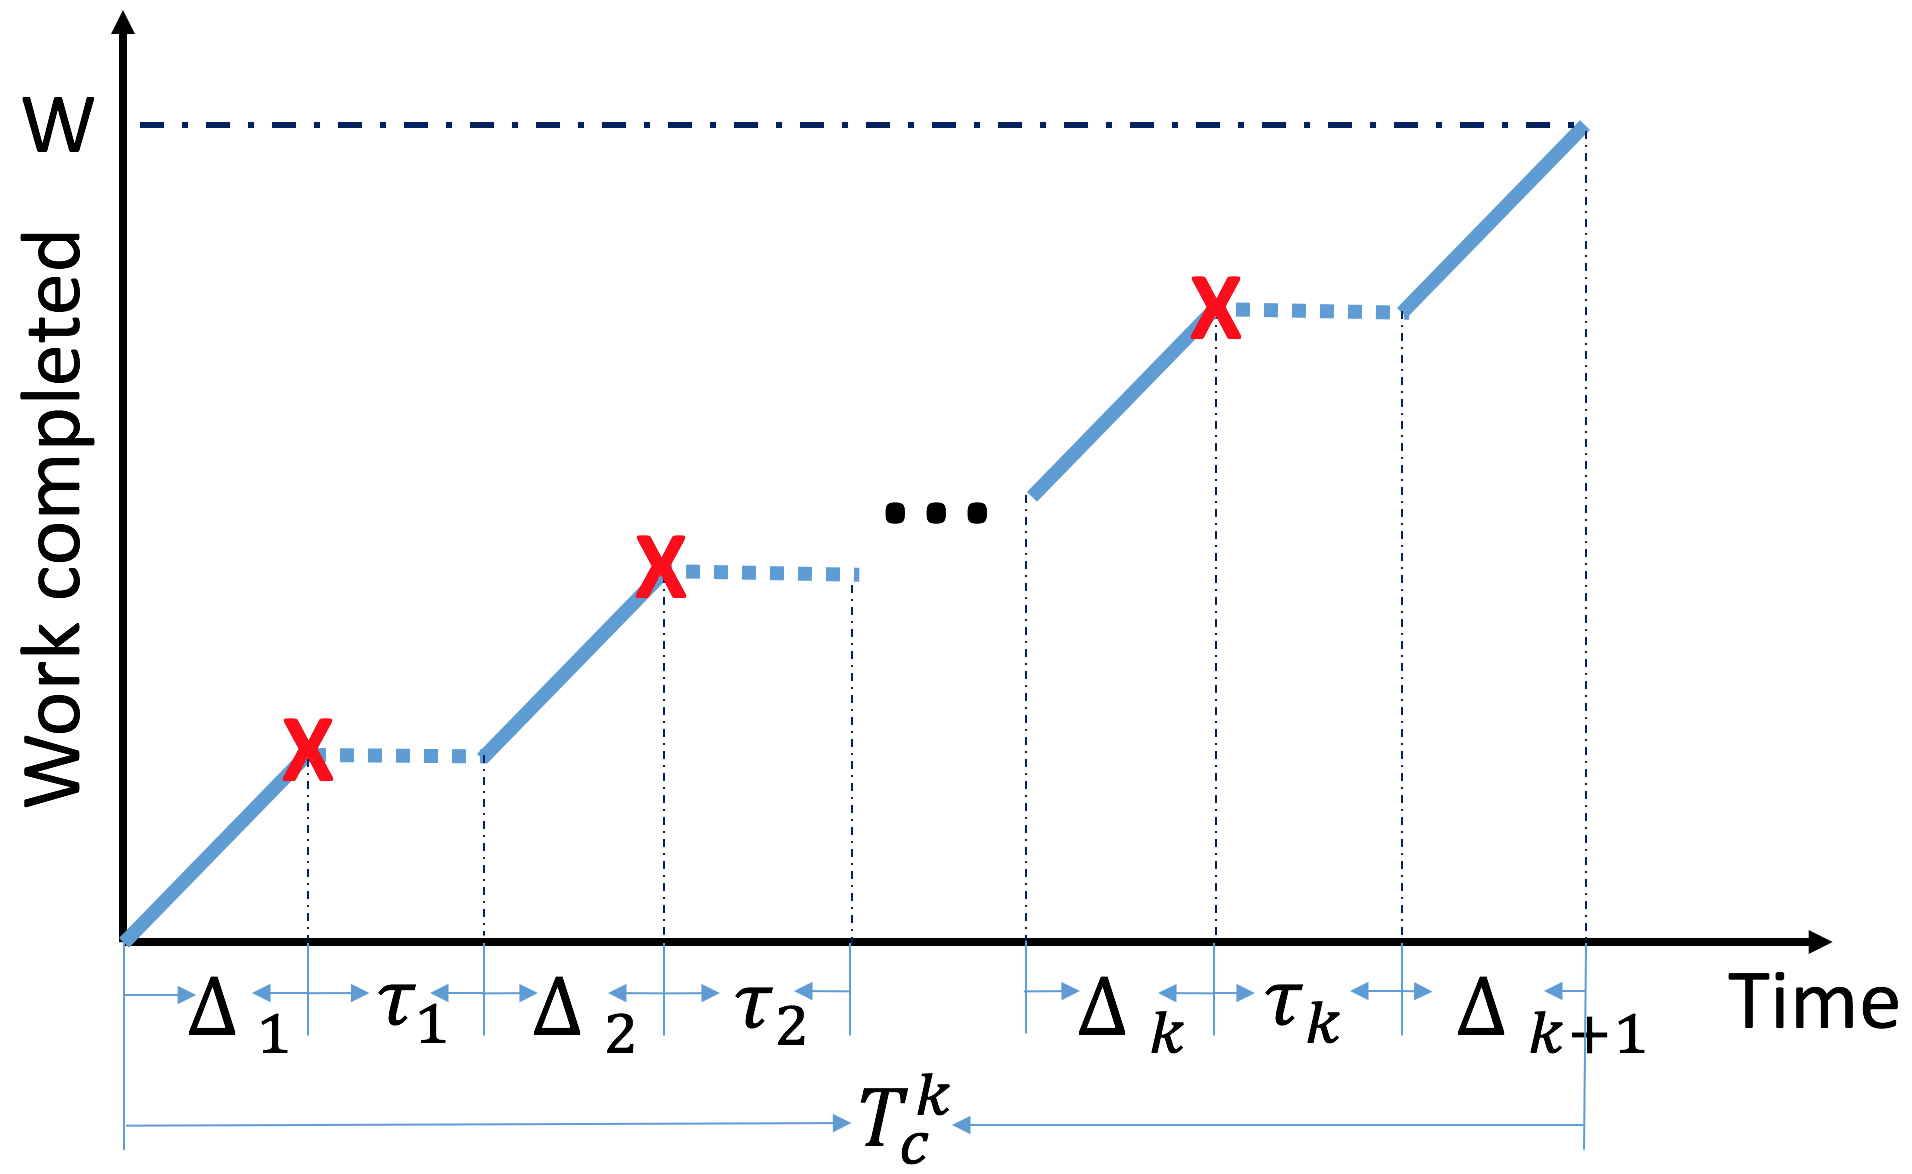
\includegraphics[width=0.7\columnwidth]{Figures/progress}
	\end{center}
	%\vskip -0.22in 
	\caption{Illustration of application's progress with failure incurred delays.}
	\label{fig:progress}
\end{figure}

Since Lazy Shadowing use $M$ cores for executing main processes and $S$ cores for shadowing ($M+S=N$), the total workload $W$ will be split into $M$ tasks, each of which will be assigned a pair of main and shadow processes. Therefore, the workload of each process is 
$w=W/M$. The following theorem gives the expression for the completion time, $T_c^k$, when there are $k$ failures.

\begin{theorem}
If no subsequent failure happens before the recovery of the previous failure, then using Lazy Shadowing, 
	$$T_c^k = w + (1-\sigma_s^b)\sum_{i=1}^k\Delta_i$$
\end{theorem}
%\begin{proof}
{\sc Proof}. The recovery time $\tau_i$ is the time needed for the lazy shadow of the failed main to catch up. Under Leaping Shadows, it is guaranteed that all the shadows reach the same execution point as the mains (See Figure~\ref{fig:leap}) after the previous recovery, so every recovery time is proportional to its previous continuous execution length, which is $\Delta_i$. That is, $\tau_i = \Delta_i \times (1 - \sigma_s^b)$ (The value of $\Delta_i$ can be obtained given a failure probability distribution, as will be demonstrated in Section~\ref{sec:evaluation}). The total delay induced by all $k$ failures is $\sum_{i=1}^k\tau_i$.
Since we assume there are $k$ failures, then $\Delta_{k+1}$ is the failure free execution interval until the workload is complete, i.e., $\Delta_{k+1} = w - \sum_{i=1}^{k}\Delta_i$. Finally, according to Figure~\ref{fig:progress}, the completion time with $k$ failures is 
	$T_c^k = \sum_{i=1}^{k+1}\Delta_i + \sum_{i=1}^k\tau_i = w + (1-\sigma_s^b)\sum_{i=1}^k\Delta_i$.
%\end{proof}
    $\square$

Although it may seem that the delay would keep deteriorating as the number of failures increases, 
it turns out to be well bounded, as a benefit of Leaping shadows:

\begin{corollary}
The delay induced by failures is bounded by $(1-\sigma_s^b)w$.
\end{corollary}
%\begin{proof}

{\sc Proof}. From above theorem we can see the delay from $k$ failures is $(1-\sigma_s^b)\sum_{i=1}^k\Delta_i$. It is straightforward that, for any non-negative integer of $k$, we have the equation $\sum_{i=1}^{k+1}\Delta_i= w$. As a result, 
$\sum_{i=1}^{k}\Delta_i = w - \Delta_{k+1} \le w$. Therefore, $(1-\sigma_s^b)\sum_{i=1}^k\Delta_i \le (1-\sigma_s^b)w$, which means the delay is bounded by $(1-\sigma_s^b)w$.
%\end{proof}
$\square$

Typically, the number of failures to be encountered will not be known before the execution. Given a failure distribution, however, we can estimate the probability for a specific value of $k$. We assume that failures do not occur during recovery, so the failure probability of a core during the execution can be estimated as $P_c = F(w)$. Then the probability that there are $k$ failures among the $N$ cores during the execution is 
\begin{equation}
\begin{split}
P_s^{k}= & \dbinom{N}{k}{P_c}^k(1-P_c)^{N-k} \\
%= & \dbinom{M}{k}({\frac{w}{MTTI}})^k(1-\frac{w}{MTTI})^{M-k}
\end{split}
\end{equation}

The following theorem gives an expression for the expected completion time, $T_{total}$, considering all possible cases of failures. 

\begin{theorem}
If no subsequent failure happens before the recovery of the previous failure, then using Lazy Shadowing,
$T_{total} = T_{c} / (1 - P_a)$, where $T_{c} = \sum_{i} T_{c}^{i} \cdot P_s^{i}$.
\end{theorem}
%\begin{proof}

{\sc Proof}. If application failure does not happen, the completion time considering all possible failures can be averaged as $T_{c} = \sum_{i} T_{c}^{i} \cdot P_s^{i}$. If application failure occurs, however, the application needs to restart from the beginning. Considering the possibility of re-execution, the total expected completion time is $T_{total} = T_{c} / (1 - P_a)$.
%\end{proof}
$\square$

Process replication is a special case of Lazy Shadowing where $\alpha=1$, so we can use the above theorem to derive the expected completion time for process replication:

\begin{corollary}
The expected completion time for process replication is $T_{total} = 2W/N / (1 - P_a)$.
\end{corollary}
%\begin{proof}

{\sc Proof}. Using process replication, half of the available cores are dedicated to replicas so that the workload assigned to each task is significantly increased given the fixed number of cores available, i.e., $w=2W/N$. Different from the case of $\alpha \ge 2$, failures do not incur any delay unless application failure occurs, since the replicas are executing at the same rate as the main processes. As a result, the completion time of process replication without application failure is constant with respect to the number of failures, i.e., $T_c^k=w=2W/N$. Therefore, the completion time, $T_c$, considering all values of $k$, is also $2W/N$. Finally, the expected completion time considering the possibility of re-execution is $T_{total} = T_c / (1 - P_a) = 2W/N / (1 - P_a)$.
%\end{proof}
$\square$

A closer look at the above analysis one can realize that Lazy Shadowing has both advantage and disadvantage compared to traditional process replication. When collocating multiple shadow processes on each core, more than half of the available cores will be dedicated to main processes, leading to less workload per process. At the same time, collocation slows down the shadow processes, which incurs delays when failures occur. We will discuss more about the conflicting effects in Section~\ref{sec:evaluation}.
 %Although it may seem that the delay would keep deteriorating as the number of failures increases, it turns out to be well bounded, as a result of shadow leaping. From Equation~\ref{eq:time_k} we can see the delay of $k$ failures is $(1-\sigma_s^b)\sum_{i=1}^k\Delta_i$. Since we have the relation $\Delta_{k+1} = w - \sum_{i=1}^{k}\Delta_i$, $\sum_{i=1}^{k}\Delta_i$ is bounded by $w$, effectively limiting the delay by $(1-\sigma_s^b)w$.

%Contrary to process replication and Lazy Shadowing, checkpointing can use all the available cores to share the total workload, so that $w = W/M$. However, the drawback is that each failure would result in an application failure which needs to roll back the execution to the last checkpoint. With that said, the recovery time of each failure is equal to the normal execution time from the last checkpoint to the time of the failure, i.e., $\tau_i = \sum_{j=1}^{i}\Delta_j$. The completion time with $k$ failures is $T_c^k = \sum_{i=1}^{k+1}\Delta_i + \sum_{i=1}^k\tau_i = w + \sum_{i=1}^{k}\sum_{j=1}^i\Delta_j$.

%\subsubsection{Expected energy consumption}







\subsection{Expected energy consumption}
\label{anal_energy}
The power consumption of one core consists of two parts, dynamic power, $p_d$, which exists only when the core is executing, and static power, $p_s$, which is constant as long as the machine is on. This can be modeled as $p = p_d + p_s$. Note that in addition to CPU leakage, other components, such as memory and disk, also contribute to static power. 

%For checkpointing and process replication, all cores are running all the time until the application is complete. Therefore, the energy consumption is proportional to the total execution time, and the expected energy consumption when using $M$ cores to execute an application is calculated as 
For process replication, all cores are running all the time until the application is complete. Therefore, the expected energy consumption, $En$, is proportional to the expected execution time $T_{total}$: 
\begin{equation}
%En = N * p * T_{total}
En = N \times p \times T_{total}
\label{eq:exp_energy1}
\end{equation} 
%Although the failed components should not consume any power, we ignore this since the number of failures is negligible compared to the total number of cores.

Lazy Shadowing has the potential to save power compared to process replication, since main cores are idle during the recovery time after each failure, and the shadows can achieve forward progress through shadow leaping. During the normal execution time, all the cores consume static power as well as dynamic power. During recovery time, however, the main cores are idle and consume only static power, while the shadow cores first perform shadow leaping and then become idle. Altogether, the expected energy consumption for Lazy Shadowing can be modeled as 
\begin{equation}
En = N \times p_s \times T_{total} + N \times p_d \times w + S \times p_{l} \times T_l.
%En = N * p_s * T_{total} + N * p_d * w + S * p_{l} * T_l.
\label{eq:exp_energy2}
\end{equation}
with $p_{l}$ denoting the dynamic power consumption of each core during shadow leaping and $T_l$ the expected total time spent on leaping. %Based on Equation~\ref{eq:exp_energy2} and Corollary 1.1, we can also establish an upper bound on the expected energy consumption for Lazy Shadowing:

%\begin{theorem}
%If no subsequent failure happens before the recovery of the previous failure, then using Lazy Shadowing, the upper bound on expected energy consumption is
%$(2N * p_s + N * p_d + S * p_{l})*w$.
%\end{theorem}
%\begin{IEEEproof}
%From Corollary 1.1 we know that the delay is at most $(1-\sigma_s^b)w \le w$, so $T_{total} \le 2w$. Also, since the leaping time overlaps with the recovery time (delay), $T_l \le (1-\sigma_s^b)w \le w$. Therefore, $En = N * p_s * T_{total} + N * p_d * w + S * p_{l} * T_l \le N * p_s * (2w) + N * p_d * w + S * p_{l} * w = (2N * p_s + N * p_d + S * p_{l})*w$.
%\end{IEEEproof}



\section{\uppercase{Evaluation}}
\label{sec:evaluation}
Extensive experiments have been done to validate our design of VTC as well as evaluate 
its performance under various scenarios. This section covers our testbeds, experiment 
methodologies, performance tuning, results, and analysis. 

\subsection{Experiment setup}
The experiments are conducted in two phases. In the first phase, only CPU is over-committed 
to validate the design of VTC with over-commitment. In this phase, we used a cluster of 18 nodes (1 login node, 1 management node, and 16 compute nodes) to mimic a realistic HPC computing environment. Each node has dual 10-core Intel Xeon E5-2660 processor and 128 GB DDR4 memory. %, and 10 Gb Ethernet. 
The hypervisor used is VMware ESXi 6.5, OS is CentOS 7.3, and resource manager is TORQUE 6.1 with the default job scheduler. We use compute-intensive benchmarks from PolyBench/C 3.1 and BioPerf~\cite{1526013}. 
In the second phase, we evaluate the full-fledged VTC design with both CPU and memory over-commitment on another testbed with huge memory capacity for memory-intensive workloads. The second cluster has 1 login, 1 management, and 8 compute nodes. Each node has dual 16-core Intel Xeon Gold 6130 processor and 768 GB memory. %, and 10 Gb Ethernet. 
The hypervisor used is VMware ESXi 6.7, OS is CentOS 7.6, and resource manager is TORQUE 6.1 with the default job scheduler. We add memory-intensive benchmarks from HPCC~\cite{dongarra2004introduction}.

\subsection{CPU over-commitment}
For performance evaluation, each node is installed with two execution environments on two separate booting disks, that is, a native OS and an ESXi hypervisor. With the hypervisor, we further define three VTC scenarios: 1) one virtual cluster; 2) two virtual clusters; 3) four virtual clusters. The latter two scenarios have 2X and 4X CPU over-commitment, respectively. 
When comparing performance among different execution scenarios (including bare metal cluster), we run the same job stream which consists of 3248 jobs that are randomly sampled from the PolyBench and BioPerf suites, and the wall clock execution time is shown in Figure~\ref{fig:cpu_exe_time}.

\begin{figure}[!t]
   \begin{center}
       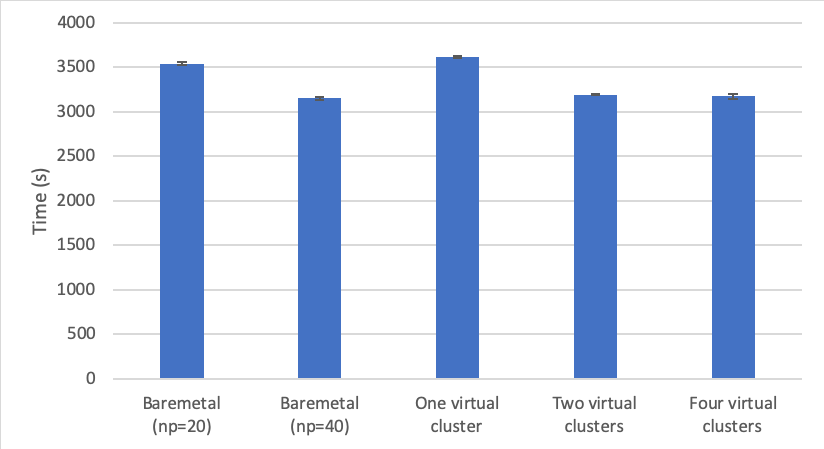
\includegraphics[width=\columnwidth]{Figures/cpu_exe_time}
   \end{center}
   \caption{Comparison of wall clock execution time for a job stream between bare metal and VTC with different CPU over-commitment ratios. Results are average of three runs.}
   \label{fig:cpu_exe_time}
 \end{figure}

Because each node in our testbed has 20 cores, in the first experiment we configured each TORQUE worker with 20 job slots. As reflected in Figure~\ref{fig:cpu_exe_time}, the execution with one virtual cluster is very close to that of bare metal (first column), with only a 2.2 percent overhead. Furthermore, when multiple virtual clusters are used with CPU over-commitment, the execution time is surprisingly shorter, implying an improved throughput despite the virtualization overhead. Through careful analysis, we identified that the throughput improvement can mainly be attributed to increased CPU utilization when more jobs are concurrently scheduled to execute. This has been verified by modifying each TORQUE worker in the bare-metal environment to use 40 job slots, after which the throughput is improved to the same level as the over-committed virtual environment. This can be seen in the second column of Figure~\ref{fig:cpu_exe_time}.

Besides execution time, another performance metric that we monitored is the total CPU utilization across the whole cluster. On the ESXi hypervisor, we used esxtop running on each compute node to sample CPU utilization of all VMs at 5-second intervals, and the results for one, two, and four virtual clusters are shown in Figure~\ref{fig:cpu_utilizations}. With two and four virtual clusters, the decreasing trend at the end is due to job completion. Clearly, CPU utilization is consistent with the job execution times in Figure~\ref{fig:cpu_exe_time}. For example, the lowest CPU utilization case--one virtual cluster--matches the longest job execution time. The higher CPU utilization with two and four virtual clusters is due to resource consolidation brought about by virtualization. That is, when multiple virtual clusters share a physical cluster, the CPU scheduler on each ESXi host has more jobs to schedule and is therefore able to make better scheduling decisions by taking advantage of Hyper-Threading and eliminating idle cycles. At the same time, improved utilization comes with better consistency, where the utilization with two and four virtual clusters is much smoother than in the single-cluster case.

\begin{figure}[!t]
   \begin{center}
       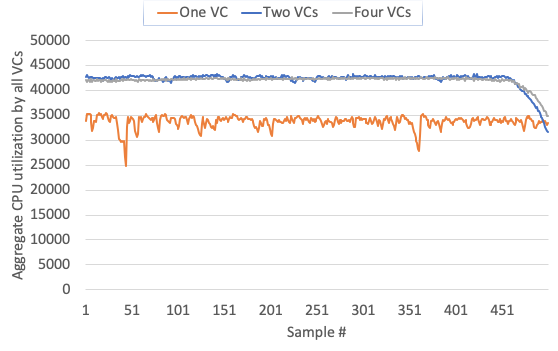
\includegraphics[width=\columnwidth]{Figures/cpu_utilizations}
   \end{center}
   \caption{Aggregate CPU utilization across 16 nodes at 5-seconds intervals.}
   \label{fig:cpu_utilizations}
   \vspace{-0.2in}
 \end{figure}

 In a production cloud environment, an important principle is fairness when multiple tenants are sharing the computing resources. We further examined the per-cluster CPU utilization in the multiple-cluster cases, and the case of four virtual clusters is shown in Figure~\ref{fig:per_cluster_utilization}. It is clear that the ESXi scheduler effectively maintains fairness so that each virtual cluster gets the same amount of CPU resources. The case of two virtual clusters is 
 the same thus not discussed. 


\begin{figure}[!t]
   \begin{center}
       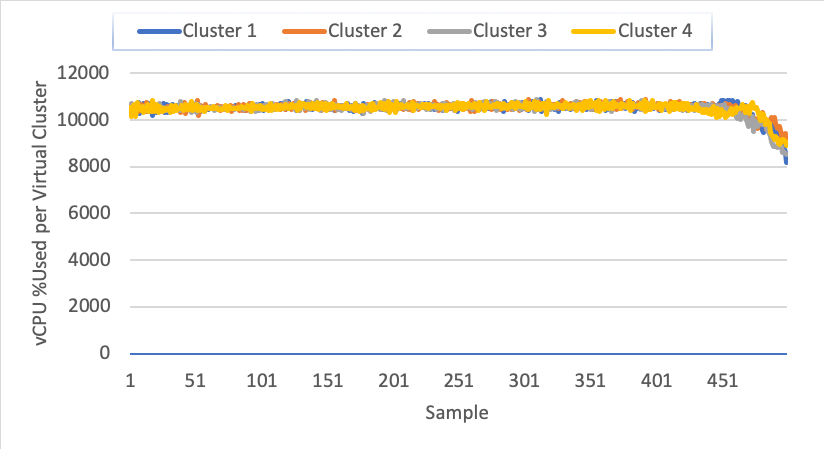
\includegraphics[width=\columnwidth]{Figures/per_cluster_utilization}
   \end{center}
   \caption{Plot of CPU utilization per virtual cluster at 5-seconds intervals for fairness check.}
   \label{fig:per_cluster_utilization}
   \vspace{-0.2in}
 \end{figure}

\subsection{CPU over-commitment with shares}
In addition to the option of equally sharing resources, the proportional, share-based scheduler of the ESXi hypervisor offers a very useful degree of flexibility. This subsection continues the CPU over-commitment study by configuring virtual clusters with different shares, to demonstrate the capability of creating a multi-tenant environment with quality-of-service guarantees. 

With the use of CPU shares, each VM can be given a particular guaranteed share of CPU resources. When there are multiple VMs running on an ESXi host, the ESXi scheduler allocates CPU based on the ratio of shares among all the running VMs. This feature extends to a virtualized HPC cloud. Specifically, each user or group can be given an appropriate share of the physical system when their virtual cluster is allocated. In this experiment, we focus on the case of four virtual clusters and set the shares ratio among the four VMs as 2:1:1:1 on every compute node. The CPU utilization is shown in Figure~\ref{fig:share_utilization}. Clearly, the CPU utilization ratio among the virtual clusters is the same as the specified shares ratio. Another important observation is that the aggregate CPU utilization across 4 virtual clusters is the same as previous no-shares case as depicted in Figure~\ref{fig:cpu_utilizations}.


\begin{figure}[!t]
   \begin{center}
       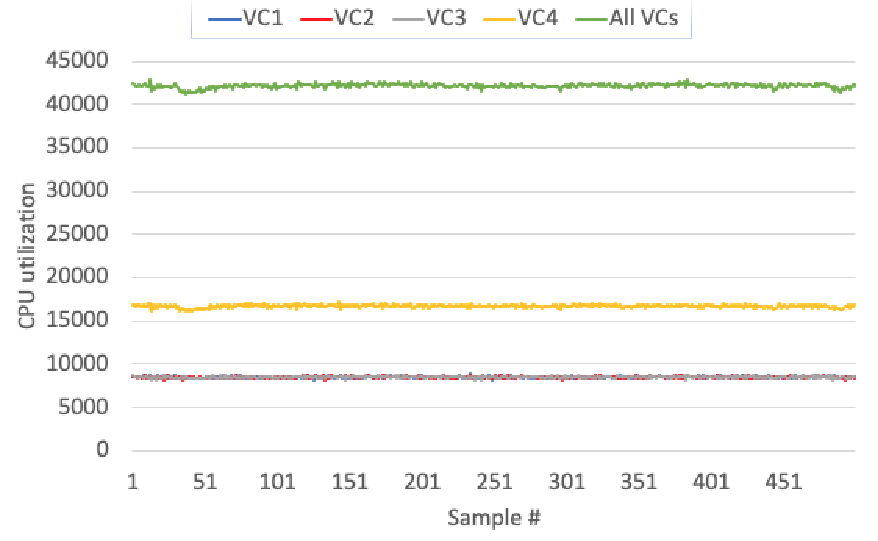
\includegraphics[width=\columnwidth]{Figures/share_utilization}
   \end{center}
   \caption{CPU utilization for four virtual clusters with 2:1:1:1 CPU shares. Utilization is sampled at 5-second intervals.}
   \label{fig:share_utilization}
 \end{figure}

\subsection{CPU + memory over-commitment}
Given that memory over-commitment is more challenging, we only test two virtual clusters with 2X CPU and memory over-commitment. vSphere Dynamic Resource Scheduler (DRS) is used to dynamically control VM migration for load balancing~\cite{infrastructure2006resource}. Considering the VM migration cost, we decided to use four quarter-size VMs to replace the single full-size VM on each node for each tenant. As a result, each tenant in this experiment gets a virtual cluster of 32 VMs across the 8 node cluster. 

To stress the system memory, we added benchmarks from HPCC. For all these HPCC benchmarks, a problem size of 53664 is chosen to have the memory consumption ranging from 16 GB to 22 GB per job instance. All the benchmarks are run with a single threaded process to mimic throughput workloads. 
To model a real HPC tenant, we specify the job arrival time to follow a Gamma distribution based on the study of several production HPC systems~\cite{lublin2003workload}.  
The resulted mean job inter-arrival time is 20.88 seconds
%The Gamma distribution has a shape parameter of 10.23 and scale parameter of 0.49. With those parameters, the mean job inter-arrival time is 10.23 / 0.49 = 20.88 seconds. 
%Also, all job sequences are shuffled to generate randomized job streams. Then, two execution scenarios are designed to represent different workload patterns. 

Two execution scenarios are designed to represent different workload patterns. In the first scenario, 1600 HPCC jobs (memory-intensive) are submitted to the first virtual cluster all at the beginning, while 1500 BioPerf jobs (memory-light) arrive at the second virtual cluster following the above Gamma distribution. The number of jobs are determined to let the two virtual clusters finish at roughly the same time. In the first virtual cluster, all the job slots will be consumed immediately and the jobs will maximize their utilization of the cluster's CPU and memory resources. In the second cluster, CPU and memory load will gradually build up. 
We make the second scenario more demanding by running two HPCC streams of 1600 jobs following the Gamma distribution. 
%Were all job slots being used, the active memory consumption would largely exceed the physical memory capacity. 
It's demanding because, even if each job only consumes 16 GB memory, 64 job instances on each node will require 64 * 16 GB = 1024 GB, which is much larger than the node capacity. It is well understood that ESXi cannot support that kind of memory over-usage. But, it is still worthwhile to explore in the realistic case where jobs randomly come and go, whether DRS can collaborate with ESXi memory reclamation techniques to accommodate this usage pattern. 

In each scenario, we run w/ and w/o DRS and measure two metrics: 1) wall clock time (WCT), i.e., the elapsed time from the start of job submission to the completion of the last job; 2) cumulative job execution time (CJET), i.e., the cumulative sum of all job instances' execution time. 

%The first metric is a measure of the system throughput, and the second metric indicates system efficiency. 
The results in scenario 1 are plotted in Figure~\ref{fig:memory_scenario1}. As the figures suggest, while VTC successfully supported 2X CPU and memory over-commitment regardless of DRS, DRS reduces HPCC's WCT by 11.1\%, which is a great improvement in throughput. 
The reason why DRS doesn't reduce BioPerf's WCT is that BioPerf jobs strictly follow the Gamma distribution in job arrivals.
But as we can see in Figure~\ref{fig:memory_cjet}, DRS reduces BioPerf's CJET by 18.4\%, making room available for more jobs. HPCC's CJET slightly increases with DRS and it indicates that DRS can cause minimal overhead to individual jobs due to telemetry sampling and VM migration. 
%, but increases HPCC CJET by 1.1\%, which is negligible. 
The number of VM migrations in each run is in the range of 30-40. It's interesting to notice that all migrations happened to the BioPerf VMs, which is because BioPerf VMs have smaller memory footprint and are lighter to migrate.

\begin{figure}
     \centering
     \begin{subfigure}[b]{0.45\textwidth}
         \centering
         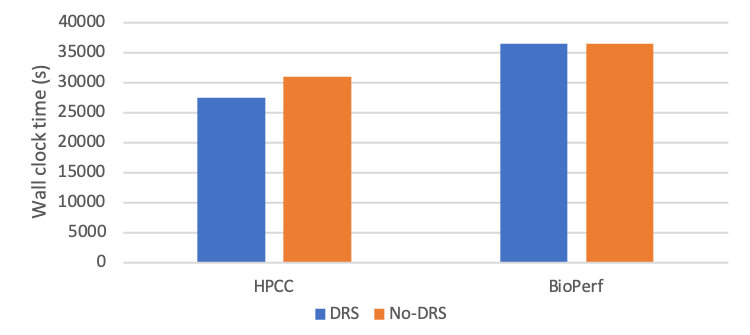
\includegraphics[width=\textwidth]{Figures/memory_wct}
         \caption{Wall clock time}
         \label{fig:memory_wct}
     \end{subfigure}
     \hfill
     \begin{subfigure}[b]{0.45\textwidth}
         \centering
         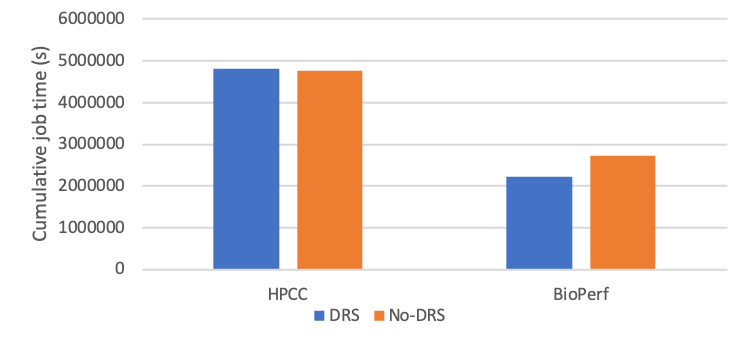
\includegraphics[width=\textwidth]{Figures/memory_cjet}
         \caption{Cumulative job execution time}
         \label{fig:memory_cjet}
     \end{subfigure}
     \caption{Comparison between DRS enabled and DRS disabled for VTC with 2X CPU and memory over-commitment. Workloads are from scenario 1. }
     \label{fig:memory_scenario1}
\end{figure}

As mentioned above, the second scenario is much more demanding because HPCC jobs can potentially consume all the configured VM memory. It's not a surprise the cluster is not able to finish two simultaneous streams of HPCC jobs, regardless of whether DRS is used. The guest OS encountered CPU soft lockup errors when hypervisor swapping occurs and when swapping is not responsive enough. Our analysis identified HPL (one benchmark in the HPCC suite) jobs as the bottleneck. Each HPL job needs more than 3 hours to finish, and once enough HPL instances accumulate on any node, the hypervisor is not able to handle their excessive memory requirements. Therefore, we decided to remove HPL from the job stream. After this change, we see that two HPCC streams can finish when DRS is on. Without DRS, the same failure occurs. Clearly, this demonstrates the effectiveness of DRS in load balancing and mitigating memory pressure. 

Though HPCC VMs are heavier to migrate, on average 67 VM migrations occurred per run, due to the extreme memory stress. Naturally, one may concern that the large number of migrations could introduce jitters to the running workloads. To quantify that, we collect the execution time distribution among all instances for each benchmark. It turns out that the execution time is quite consistent. For example, the histogram for RandomAccess (another benchmark in the HPCC suite) is shown in Figure~\ref{fig:ra_histogram}.

\begin{figure}[!t]
   \begin{center}
       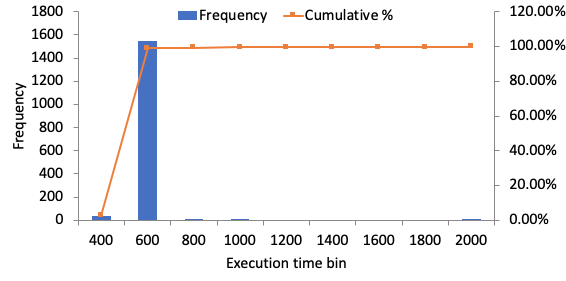
\includegraphics[width=\columnwidth]{Figures/ra_histogram}
   \end{center}
   \caption{Histogram of individual RandomAccess job execution time from both virtual clusters.}
   \label{fig:ra_histogram}
 \end{figure}






\section{\uppercase{Conclusion}}
\label{sec:conclusion}
%Current fault-tolerance approaches rely exclusively on either time or hardware redundancy for recovery. Rollback recovery  exploits time redundancy but can incur significant delay and high energy cost. On the other hand, process replication relies on hardware redundancy and requires a significant increase in resources and  power consumption.

In this paper, we propose Rejuvenating Shadows as a novel power-aware fault tolerance model, which guarantees forward progress, maintains consistent level of resilience, and minimizes implementation complexity and runtime overhead. Empirical experiments demonstrated that the Rejuvenating Shadows model outperforms in-memory checkpointing/restart in both execution time and resource utilization, especially in failure-prone environments.

Leaping induced by failure has proven to be critical in reducing the divergence between a main and its shadow, 
%with respect to workload execution.
%Consequently, the time to recover from subsequent failures is reduced significantly. 
thus reducing the recovery time for subsequent failures. Consequently, the time to recover from a failure increases with failure intervals.  
Based on this observation, a proactive approach is to ``force" leaping when the divergence between a main and its shadow exceeds a specified threshold. 
In our future work, we will further study this approach to determine what behavior triggers forced leaping in order to optimize the average recovery time. 

%we will study forcing the shadDuring experimentation we noticed the problem that recovery time in Rejuvenating Shadows can become substantial when the failure interval is large (Figure~\ref{fig:single_failure}). To deal with this issue, we are studying the idea of ``forced leaping", which borrows the idea from periodic checkpointing and forces a leaping whenever failure has been absent for a long time, in order to reduce the divergence between mains and shadows. Optimal intervals for forced leaping will be explored to balance between runtime overhead and failure recovery overhead. 

%In the future we plan to explore the integration with fault prediction techniques and the viability of dynamic and partial shadowing for platforms where nodes exhibit different ``health" status, e.g., some nodes may be more reliable while others are more likely to fail~\cite{gainaru2012fault}. 
%With this taken into account, we can apply dynamic scheduling of shadows only for mains that are likely to fail, to further reduce the resource requirement. 
%Another future direction is to study complier-assisted program slicing for fault detection. Specifically, slices that are fraction of their mains can run lazily as shadows and provide fault detection capability with reasonable coverage. 






% trigger a \newpage just before the given reference
% number - used to balance the columns on the last page
% adjust value as needed - may need to be readjusted if
% the document is modified later
%\IEEEtriggeratref{8}
% The "triggered" command can be changed if desired:
%\IEEEtriggercmd{\enlargethispage{-5in}}

% references section

% can use a bibliography generated by BibTeX as a .bbl file
% BibTeX documentation can be easily obtained at:
% http://www.ctan.org/tex-archive/biblio/bibtex/contrib/doc/
% The IEEEtran BibTeX style support page is at:
% http://www.michaelshell.org/tex/ieeetran/bibtex/
%\bibliographystyle{IEEEtran}
% argument is your BibTeX string definitions and bibliography database(s)
%\bibliography{IEEEabrv,../bib/paper}
%
% <OR> manually copy in the resultant .bbl file
% set second argument of \begin to the number of references
% (used to reserve space for the reference number labels box)

%\begin{thebibliography}{1}
%
%\bibitem{IEEEhowto:kopka}
%H.~Kopka and P.~W. Daly, \emph{A Guide to \LaTeX}, 3rd~ed.\hskip 1em plus
%  0.5em minus 0.4em\relax Harlow, England: Addison-Wesley, 1999.
%
%\end{thebibliography}



\bibliographystyle{IEEEtran}
\bibliography{IEEEabrv,main}  



% that's all folks
\end{document}


